\documentclass[12pt]{article}
\usepackage[utf8]{inputenc}
\usepackage{amsmath}
\usepackage{makebox}
\usepackage{amssymb}
\usepackage{amsthm}
\usepackage{graphicx} % graficos
\usepackage{fullpage}
\usepackage{fancyhdr}
\setlength{\parskip}{0.2pt}
\usepackage{hyperref}
\usepackage{xcolor}
\usepackage{subcaption}
\usepackage{listings}
\usepackage{marvosym}
\usepackage{float}

\begin{document}
\lhead{\begin{picture}(0,0) \put(0,0){
\includegraphics[width=25mm]{U}} \end{picture}}

\rhead{\begin{picture}(0,0) \put(-59,0){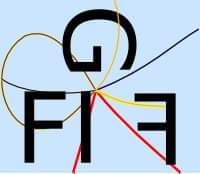
\includegraphics[width=25mm]{gfif.jpeg}} \end{picture}}
\pagestyle{fancy}




\begin{center}
    \Large \textbf{Generación de masas de neutrinos}. \normalsize
\end{center}

\begin{center}
    Kimy Johanna Agudelo Jaramillo  \\
    Grupo  de Fenomenología e Interacciones Fundamentales.
\end{center}

%------------------------------------------------------------------
\section{Introducción}
% En el presente trabajo pretendemos desarrollar un modelo ....que permitan construir ...... en el ME
%
La historia de los neutrinos se remonta al año 1896, cuando Henri Becquerel, Pierre y Marie Curie descubrieron las radiaciones provenientes del uranio y radio. En 1899, Ernest Rutherford descubrió las radiaciones alfa y beta, un año más tarde Paul U. Villard descubrió la radiación gamma. Pocos años despúes, las radiaciones alfa, beta y gamma fueron identificados como núcleos de helio, electrones y fotones respectivamente.

En el año 1914, James Chadwick demostró que el espectro beta es continuo, lo que implica la violación del principio de conservación de la energía$^{[1]}$. Dicho descubrimiento fue confirmado por Ellis y Woostee en 1927. En ese entonces, la radiación beta se asumía como la emisión de un solo tipo de partícula (el electrón), por lo tanto, esta debía tener una energía bien definida. Lise Meitner experimentalmente, descubrió que la falta de energía no podía atribuirse a los rayos gamma neutros.
 Wolfgang Pauli en 1929 postula la existencia de una partícula neutra para sostener el principio de conservación de la energía en el decaimiento beta y la cual Enrico Fermi  nombró neutrinos,  de espín $\frac{1}{2}$  y con una masa muy por debajo a la del electrón e incluso con la posibilidad de que fuera nula.
 
 En 1934 Fermi formula una teoría que describe el proceso del decaimiento beta$^{[3]}$.Los neutrinos y antineutrinos de tipo electrónico se producen en desintegración $\beta^{\pm}$ nuclear, a partir de la siguiente interacción: $n = p + e^- + \bar{\nu}_R$. 

 Por medio de la reacción de un material rico en protones en 1956, F. Reins y C. Cowan  confirmaron la existencia del neutrino, en la cuál se producían neutrones y positrones debida a la emisión de neutrinos electrónicos provenientes de un reactor nuclear.$^{[1]}$
 En el experimento Super Kamiokande se detectan neutrinos mediante dispersión elástica de electrones por neutrinos a partir del efecto Cherenkov. Se determinó la existencia de tres variedades de neutrinos, neutrino electrónico $\nu_e$, muónico  $\nu_\mu$ y tauónico $\nu_\tau$, cada neutrino asociado a una familia de leptones cargados.

Ahora se tiene la evidencia de que los neutrinos interactúan muy débilmente a través de la interacción débil, la cual está descrita en el Modelo Estándar (SM).  Aunque el Modelo Estándar (SM) ha sido exitoso en la predicción de muchos parámetros experimentales, engloba un conjunto de aspectos, en su mayoría teóricos a los que no responde de manera satisfactoria. Uno de los problemas más interesantes del SM es la ausencia de masa de los neutrinos, lo cual se contradice con la evidencia experimental. Se ha establecido que los neutrinos tienen masa pequeña, pero distinta de cero, por lo tanto se genera la primera prueba experimental de una nueva física más allá del Modelo Estándar.\\ 
 
 Esté descubrimiento ha revolucionado enormemente la actividad teórica intentando descubrir la naturaleza de esta nueva física. Por lo que se requiere de modelos más allá del SM; como modelos en que se extiende la estructura de simetría del SM a grupos más grandes, por ejemplo en el caso de modelos de unificación y modelos con la misma estructura de grupo del SM, que extienden su contenido de partículas en su sector fermiónico, o escalar.$^{[5]}$ 

Otro interrogante concerniente a los neutrinos masivos es su naturaleza. ¿Los neutrinos son partículas de Dirac o de Majorana?. Los neutrinos pueden ser partículas Dirac, cómo lo son todos los fermiones cargados. Sin embargo existe la posibilidad de que los neutrinos sean sus propias antipartículas ya que estos no poseen carga eléctrica.  \\

Una alternativa interesante para introducir la masa de los neutrinos al SM son los llamados mecanismos Seesaw, con lo cuál se podría explicar de forma natural el pequeño valor que toman las masas de los neutrinos. Dichos mecanismos se presentan en tres formas diferenciadas$^{[2]}$: Tipo I, Tipo II y Tipo III. Cada forma incluye extensiones del Modelo Estándar con una nueva escala de energías más allá de la electrodébil y que dan cuenta de la masa del neutrino.

\subsection{\textbf{El Neutrino en el Modelo Estándar Minimal}} El modelo estándar de física de partículas es una teoría cuántica de campos relativista que describe la estructura fundamental de la materia y el vacío, las partículas en éste modelo son consideradas como elementos irreducibles cuyo movimiento en el espacio-tiempo (cinemática) se encuentra regida por tres de las cuatro fuerzas fundamentales, la fuerza fuerte, fuerza débil y electromagnética (Se excluye la gravedad, ya que la relatividad general no se acopla con los modelos cuánticos).


\begin{itemize}
\item \textbf {El Modelo Estándar Electrodébil:} dicho modelo corresponde al  sector \(SU(2)_L\otimes U(1)_Y \rightarrow U(1)_Q \) el cual describe el espectro físico de partículas una vez se ha implementado la Ruptura Espontánea de la Simetría

\begin{equation}
\fbox{$SU(2)_L\otimes U(1)_Y \rightarrow U(1)_Q$ }
\label{eq:1}
\end{equation} 

\begin{itemize}
\item \(U(1)_Q \rightarrow \) Interacción electromagnética mediada por fotones. %(\(\nu \))
\end{itemize} 
\end{itemize} 

%---------------------------------------------------------------------

\subsection{Teoría Lagrangiana}


La Teoría Cuántica de Campos (TCC) es el marco teórico utilizado en la descripción cuántica de campos relativistas. Dicha teoría surgió de acoplar la mecánica cuántica con la relatividad especial en un marco consistente. Las teorías cuánticas de campos se describen más convenientemente en el formalismo Lagrangiano. De hecho, los Lagrangianos que describen las partículas elementales y sus interacciones puede ser construidos a partir de principios de simetría.$^{[5]}$ \\


A continuación, se hacen presentes los métodos variacionales para obtener la variación de la acción debida a transformaciones de los campos $\psi_i$. Con el resultado de está variación se obtiene la ecuación de Euler-Lagrange para luego pasar al Teorema de Noether. 

\subsubsection{Principio variacional y teoría de campos}

Consideremos un conjunto de $n$ campos reales $\psi_i(x)$, con $i=1,2,...,n$. Un campo es un conjunto de números en cada punto en el espacio-tiempo. La descripción del lagrangiano real viene dada por: 

\begin{equation}
    \mathcal{L}(x)= \mathcal{L}(\psi_i(x), \partial_\mu\psi_i(x))
\end{equation}

\begin{itemize}
\item El lagrangiano no debería depender explícitamente de las coordenadas espacio-temporales.

\end{itemize}

Para el estudio de las teorías del campo relativista resulta conveniente utilizar el formalismo del lagrangiano, debido a que es un escalar de Lorentz (además del hecho que estamos interesados en campos fundamentales),  mientras que el hamiltoniano representa la energía de los campos y se transforma como la componente temporal de la energía-momento de cuatro vectores. \\ 

Se quiere describir éste sistema por una acción, la cual va estar escrita como una integral temporal del lagrangiano. Entonces finalmente podemos escribir la acción en la forma

\begin{equation}
    \mathcal{A}(\Omega) \equiv \int_\Omega dx^4 \mathcal{L}(\psi_i(x), \partial_\mu\psi_i(x))
\end{equation}

\begin{itemize}
    \item $dx^4 \rightarrow  $ Elemento de volumen espacio-temporal.
\end{itemize}

Donde $\Omega$ es una región arbitraria del espacio-tiempo (región en la cual estamos interesados). Según el principio variacional, los campos deben ser tales que la acción sea estacionaria, por lo tanto: 

\begin{equation}
  \delta_v \mathcal{A}(\Omega)=0  
\end{equation}

Para variaciones infinitesimales de los campos que se desvanecen en la hiperesuperficie S que rodea la región espacio-temporal $\Omega$. Estás variaciones son del tipo

\[ \psi_i(x) \rightarrow \psi_i(x) + \delta_v  \psi_i(x) \]
\begin{equation}
\partial_\mu\psi_i(x) \rightarrow \partial_\mu\psi_i(x) + \partial_\mu \delta_v  \psi_i(x)
\label{equ:variacion}
\end{equation} \\

La variación de la acción bajo la transformacion en (\ref{equ:variacion}) viene dada por: 

%
\begin{equation}
  \delta_v \mathcal{A}(\Omega)=  \int_\Omega dx^4  \sum_{i}\left[\frac{\partial\mathcal{L}}{\partial\psi_i}\delta_v\psi_i + \frac{\partial\mathcal{L}}{\partial(\partial_\mu\psi_i)}\delta_v(\partial_\mu\psi_i)\right] 
\end{equation} \\

Después de desarrollar y utilizar el Teorema de Gauss se obtiene,

\begin{equation}
    \delta_v \mathcal{A}(\Omega)= \int_\Omega dx^4  \sum_{i}\left[\frac{\partial\mathcal{L}}{\partial\psi_i} - \partial_\mu  \frac{\partial\mathcal{L}}{\partial(\partial_\mu\psi_i)}\right]\delta_v\psi_i   =0
\end{equation} \\ 

Dado que las variaciones $\delta_v  \psi_i(x)$ son arbitrarias e independientes para diferentes $ n $, los campos $\psi_i(x)$ deben satisfacer la \textit{Ecuación de Euler-Lagrange } 
 
 \begin{equation}
\frac{\partial\mathcal{L}}{\partial\psi_i} - \partial_\mu  \frac{\partial\mathcal{L}}{\partial(\partial_\mu\psi_i)}=0 \quad (i=1,2,...n)
\label{equ:Euler-Lagrange}
 \end{equation} \\


 Está claro que el carácter escalar del lagrangiano es crucial para garantizar la covarianza de Lorentz de las ecuaciones de campo en la ecuación (\ref{equ:Euler-Lagrange})
 
%-----------------------------------------------------------------

\subsubsection{Teorema de Noether}

Asociado con cada simetría de un sistema hay una cantidad conservada. Por lo tanto, si conocemos algunas cantidades conservadas de un sistema, podemos trabajar hacia atrás para encontrar las simetrías del sistema y, a partir de ahí, adivinar la forma de un adecuado Lagrangiano. El resultado que relaciona las simetrías con las cantidades conservadas se conoce como teorema de Noether. 

\subsubsection{Campos complejos}

Sí los campos $\psi_i$ son complejos, cada campo tiene dos grados de libertad que pueden ser representados por una parte real y una parte imaginaria, $\psi_i$ y $\psi_i^ *$ (o $\psi_i^\dagger$ en el caso de campos cuantizados ) respectivamente. 

%------------------------------------------------------------------
\section{Simetrías y rupturas de simetría}

Las simetrías tienen consecuencias importantes en cualquier teoría cuántica de Campos (TCC). Pueden encontrar ``masas o energías"
de diferentes estados, o dispersión de secciones transversales de diferentes procesos. 

\subsection{Simetrías globales}

Según el teorema de Noether, la conservación de la carga es una consecuencia de la invariancia del lagrangiano $\delta \mathcal{L}=0 $ bajo las transformaciones de fase de los campos complejos,dichas transformaciones reciben el nombre de \textit{transformaciones globales}, 

\begin{equation}
   \fbox{ $ \psi_i(x) \rightarrow e ^ {i\theta}\psi_i(x)$}
   \label{eq:gaugeglobal}
\end{equation} 
donde, $\theta $ es un parámetro arbitrario,  Las cargas conservadas más conocidas son la carga eléctrica y los números bariónicos y leptónicos.\\  

La transformación global (donde, \textit{global} nos indica que el parámetro $\theta$ no depende del espacio-tiempo) en la ecuación (\ref{eq:gaugeglobal}) implica una variación común de las fases de todos los $n$ campos $\psi_i(x)$. Tal transformación pertenece al grupo abeliano U(1) de transformaciones de fase continua. 

\subsection{Simetrías globales del modelo}

El modelo estándar eletectrodébil está basado en una \textit{simetría local } con el grupo gauge $\text{SU(2)} \otimes \text{U(1)}$. Evidentemente esto implica la misma simetría global. Pero además, el modelo estándar también tiene algunas otras simetrías globales.

Una de ellas, es la simetría del número bariónico, la cual está definida de la siguiente manera: 

\begin{equation}
\centering
q \rightarrow e^ {-i\mathcal{B}\theta}q
    \label{eq:numerobarionico}
\end{equation} \\ 
Donde, $q$ son todos los campos quark y $\mathcal{B}$ es el \textit{número bariónico} de los quark, generalmente se toma como $\mathcal{B}= \frac{1}{3}$. Para los antiquarks se tiene el siguiente valor, $\mathcal{B}= - \frac{1}{3}$.

Se asume que todas las otras partículas tienen un número bariónico igual a cero. Lo cual implica que no transforman bajo  la operación de simetría mostrada en la ecuación (\ref{eq:numerobarionico}). Se puede verificar además que ninguna interacción del modelo estándar cambia un quark en un leptón, de ahí esta simetría. \\ 

En el sector leptónico también hay simetrías de este tipo. Por ejemplo, considere 

\begin{equation}
\centering
l \rightarrow e^ {-i\mathcal{L}\theta}l
    \label{eq:numeroleptonico}
\end{equation} 
donde, $l$ es cualquier leptón cargado negativamente o su correspondiente neutrino y  $\mathcal{L}$ se conoce como el \textit{número leptónico}, además se toma como $-1$ para los leptones y $+1 $ para las antipartículas.

Se asume que todas las otras partículas tienen un número leptónico igual a cero. 

Estás simetrías tienen un carácter muy diferente que las simetrías gauge: 
\begin{enumerate}
\item Estás son simetrías globales, opuesto a la simetría gauge las cuales son locales. 

\item Estás simetrías no son impuestas en el modelo. Desarrollando la teoría con la simetría gauge y con el contenido específico de fermiones, se encontraron estas simetrías adicionales. Las cuales reciben el nombre de \textit{simetrías accidentales}. 

\end{enumerate}

%CARLO GUINTUI PAG 627 THE TRANSFORMATIONS NONABELIAN PILAS!!!!! 


%------------------------------------------------------------------

\section{Fenomenología de masas de neutrinos: neutrinos de Weyl, Majorana y Dirac }

Un fermión (o un neutrino sin masa) puede ser descrito mediante un campo espinor de Weyl de dos componentes (siendo está la forma mínima para introducir un fermión), componente quiral izquiera \(\psi_L\) y la respectiva componente quiral derecha \(\psi_R\); es decir que siempre es posible dividir un campo espinor de la siguiente manera:

\begin{equation}
\psi= \psi_R+ \psi_L
\label{eq:2'}
\end{equation}   

Siendo \(\psi_R\) y \(\psi_L\)  las autofunciones de la matriz \(\gamma^{5}\) con autovalores +1 y -1 respectivamente:

\begin{equation}
\gamma^{5}\psi_R= + \psi_R
\end{equation} 
\begin{equation}
\gamma^{5}\psi_L= - \psi_L
\end{equation} 
Donde los espinores de Weyl viene dados por: 

\begin{equation}
\psi_R= \frac{1+\gamma^{5}}{2}\psi=P_R\psi
\label{eq:2*}
\end{equation} 

\begin{equation}
\psi_L= \frac{1-\gamma^{5}}{2}\psi= P_L\psi
\label{eq:2**}
\end{equation} 

\begin{itemize}
    \item \(\gamma^{5} \rightarrow \) matriz de quiralidad
    \item \(P_L \) y \(P_R \rightarrow \) matrices de proyección de quiralidad
\end{itemize}


Cuando introducimos un fermión con una sola helicidad, es decir fermión izquierdo o derecho, la teoría cuántica de campos se descompensa, esto debido a que se rompe la simetría gauge de la teoría a un loop, generando anomalías en el modelo. \\

Sin embargo cuando se introducen fermiones con las dos helicidades (derecha e izquierda) se cancelan las anomalías entre sí, implicado la invarianza del modelo, el cual queda  completamente simétrico a un loop y a cualquier otro orden en teoría de perturbaciones. 


%------------------------------------------------------------------
\section{El sector escalar}

Debido a que el modelo debe contener al MEM, se debe respetar el Rompimiento Espontáneo de la Simetría (R.E.S). Por lo que, se debe implementar un sector escalar adecuado que permita el correcto rompimiento de los generadores primero al MEM y luego a la QED. Además, en las extensiones mas allá del modelo estándar mínimo se debe asegurar que el sector escalar genere masas pesadas a las partículas extras asociadas a nueva física y masas mas livianas a la escala electrodébil del espectro fenomenológico observado a bajas energías y descrito por el modelo estándar mínimal.  


\subsection{Rompimiento Espontáneo de la Simetría (R.E.S)}

Cuando se tienen modelos que describen interacciones entre partículas, (ya sea un modelo clásico o uno cuántico), surge el problema de la autointeracción, es decir, la interacción del campo producido por una partícula sobre sí misma. Al tratar de solucionar dicho problema, las ecuaciones llevan a resultados divergentes, donde la intensidad de la interacción se hace infinita. Sin embargo, esos infinitos pueden ser eliminados o anulados con la introducción de otros infinitos implementados de forma sistemática a través del mecanismo de renormalización. \\

Por lo tanto, una condición importante en cualquier modelo de partículas elementales que describa interacciones,es que pueda renormalizarse$^{[7]}$. Dicho requerimiento de renormalización debe mantenerse a todos los ordenes de corrección si se aplica teoría de perturbaciones en el modelo. Otra condición para mantener la renormalización, es evitar la introducción directa de términos de masa en el lagrangiano (términos de la forma $m\psi\bar{\psi}$ para fermiones), los cuales además dañan la invarianza gauge de la teoría. Sin embargo hay una forma indirecta de introducir ese tipo de términos, los cuales son necesarios en el modelo, ya que es evidente que la mayoría de partículas son masivas. El procedimiento es un mecanismo que rompe la simetría del vacío (no del lagrangiano) preservando aun los efectos de la invarianza, y que se implementa de tal forma que la renormalización se mantenga$^{[8]}$. 

%----------------------------------------------------------------

\subsection{Mecanismo de Higgs}

Consiste en introducir un campo escalar \(\Phi\) que interactúa con los Bosones de Gauge y Fermiones, cuyo estado de mínima energía (estado de vacío) puede presentar dos casos de simetría:

\begin{enumerate}

\item \textbf {Antes del Rompimiento Espontáneo de la Simetría:} El vacío tiene la misma invarianza de Gauge que el Lagrangiano y todas las partículas aparecen sin masa.\\ 

\item \textbf {Después del Rompimiento Espontáneo de la Simetría:} El vacío se degenera y los fermiones y algunos bosones de Gauge adquieren valores de masa que se ajustan de acuerdo con los datos experimentales.

De esta manera surge una relación entre la obtención de masa de una partícula y el rompimiento espontáneo de alguna simetría.\\

En el rompimiento de $SU(2)_L\otimes U(1)_Y  \rightarrow^\Phi U(1)_Q $ el vacío deja de ser invariante bajo los tres generadores: \(\hat{T_1}, \hat{T_2}\) y una combianción ortogonal \(\hat{Q}=\hat{T_3}+ \hat{Y}\). Esto puede expresarse de la suguiente manera,
\begin{equation}
    [{T_{1,2}}^{SU(2)}, \langle \Phi \rangle_0  ] \neq  0 
    \label{eq:2}
\end{equation}

\begin{equation}
    [{T_{3}}^{SU(2)}-\hat{Y}, \langle \Phi \rangle_0  ] \neq  0 
    \label{eq:3}
\end{equation}

\begin{equation}
    [\hat{Q}, \langle \Phi \rangle_0  ] =  0 
    \label{eq:4}
\end{equation}

Donde, 

\begin{itemize}
\item \(\hat{T} \rightarrow \) Generadores de un grupo especial unitario \(SU(2)_L\)
\item \(\hat{Q} \rightarrow \) Generador de carga eléctrica.
\item \(\hat{Y} \rightarrow \) Hipercarga \(\hat{Y} =\beta \hat{Y_0} \)
\item \(\hat{T_3} \rightarrow \) Isospín.
\item \(\langle \Phi \rangle_0  \) Valor esperado en el vacío, del campo.

\end{itemize}

De las ecuaciones (\ref{eq:2}) y (\ref{eq:3}) se obtienen 3 generadores rotos, por lo tanto hay 3 Bosones de Gauge que adquieren masa. De la ecuación (\ref{eq:4}) queda un bosón de Gauge sin masa (Fotón), el cual se considera como un generador no roto. \\ 


\begin{itemize}
\item \underline{ \textbf{Condiciones para masas de Fermiones}}: El mecanismo Higgs no implementa directamente las masas de los fermiones. Para dotar de masa a estas partículas se introducen términos de interacción entre fermiones \(\psi\) y campos escalares \(\phi\). A este tipo de
interacción se le denomina \textbf{interacción de Yukawa}. Los términos de
interacción de Yukawa que son invariantes Lorentz, hermíticos, renormalizables y que guardan simetría bajo \(SU(3)_C \otimes SU(2)_L \otimes U(1)_Y \).

Y pueden ser expresados de la siguiente manera, 

\[\bar{\psi}\psi\Phi + \bar{\psi}(\psi)^{c}\Phi +  \bar{\psi^c}(\psi)\Phi^{\dagger} + \bar{\psi^c}(\psi)^c\Phi^{\dagger} = \]
\begin{equation}
    \bar{\psi_L}(\psi_L)^{c}\Phi + \bar{\psi_L}(\psi_R)\Phi  +  \bar{\psi_R}(\psi_R)^c\Phi + \bar{(\psi_R)^c}(\psi_L)^c\Phi + \text{h.c}  
    \label{eq:5}
\end{equation}
\end{itemize}

donde h.c son los hermíticos conjugados. \\

Los términos de Yukawa deben garantizar la invarianza \(SU(2)_L\), los cuales deben formar singletes, siguiendo las siguientes condiciones:

\[\bar{\psi_L^i}\psi_R\Phi : 2^*\otimes1 \otimes n \rightarrow \fbox{$n=2$}
 \]
\begin{equation}
\label{eq:21}
    \bar{{\psi}_L^i}({\psi}_L^j)^c\Phi : 2^* \otimes 2^*\otimes n \rightarrow \fbox{$n=2\otimes 2$} \end{equation}
\[\bar{\psi_R}(\psi_R)^c\Phi : 1\otimes 1\otimes n \rightarrow \fbox{$n=1 $}\]
\begin{equation}
\bar{(\psi_L^i)^C}\psi_R\Phi : 2\otimes1 \otimes n \rightarrow \fbox{$n= 2^*$}
\label{eq:6}
\end{equation}

Es muy importante tener en cuenta que las representaciones que se elijan para las soluciones dadas en la ecuación (\ref{eq:6}) deben garantizar las siguientes condiciones:

\begin{enumerate}
\item El valor esperado en el vacío,  \(\langle \Phi \rangle_0  \) debe ser invariante bajo los tres generadores. Es decir, debe cumplir con  (\ref{eq:2}), (\ref{eq:3}) y (\ref{eq:4})

\item El número de componentes de \(\Phi  \) debe ser ajustable al número de Bosones de Goldstone.

\item El valor esperado en el vacío,  \(\langle \Phi \rangle_0  \)  cuando se reemplaza en los términos de Yukawa debe conllevar al número correcto de fermiones, los cuales adquieren masa, esto de acuerdo a la transición que se realiza en el rompimiento espontáneo de la simetría (R.E.S). 
\end{enumerate}

%--------------------------------------------------------------------
\section{Modelo con el Triplete de Higgs}

Uno de los mecanismos para generar masas de neutrinos consiste en expandir el sector escalar mediante la introducción de un triplete de Higgs. Este modelo proporciona masas de Majorana para los neutrinos sin necesidad de postular neutrinos derechos vía la interacción de Yukawa. El Lagrangiano de Yukawa con el triplete de Higgs toma la siguiente forma:

\begin{equation}
    \mathcal{L}= \frac{1}{\sqrt{2}} \sum_{n,m=1}^3 Y^{nm} \bar{\psi_L^{ni}}\tau \cdot \triangle^{'} ({\psi_L^{mj}})^{c} + \text{h.c} 
    \label{eq:7}
\end{equation} 

El modelo incorpora nuevas partículas en el Modelo Estándar: un bosón de Higgs doblemente cargado \(\triangle^{++} \), un bosón simplemente cargados, \(\triangle^{+} \) y un bosón de Higgs neutro \(\triangle^{0} \). 

A continuación se muestra el espectro del Modelo con las correspondientes partículas: 


\begin{enumerate}
\item \underline{ \textbf{Fermiones:}}

Cuando se añade un doblete de Higgs al Modelo Estándar se permite que algunos fermiones y bosones electrodébiles adquieran masa, sin embargo esto no permite que los neutrinos adquieran masa, por lo tanto se hace necesario que se añada el triplete de Higgs. \\ 

\begin{itemize}
\item \textbf{Fermiones izquierdos:} 
\end{itemize}

\begin{equation}
\begin{aligned}
      l_{L^{(n)}} & = \binom{\nu^{(n)}}{e^{(n)}}_L = \begin{pmatrix}  \nu_e & \nu_\mu & \nu_\tau \\ e &  \mu &  \tau \end{pmatrix}_L & :  (\textbf{2}, -1/2)  
\end{aligned}
\end{equation}
\begin{equation}
\begin{aligned}
   q_L^{(n)} & = \binom{u^{(n)}}{d^{(n)}}_L  & = \begin{pmatrix} u & c & t \\ d &  s  &  b \end{pmatrix}_L & :  (\textbf{2}, 1/6) \\ 
\end{aligned}
\end{equation} \\

\begin{itemize}
\item \textbf{Fermiones derechos:}
\end{itemize} 

\begin{equation}
 e_R^{(n)} = e_R, \mu_R , \tau_R: (\textbf{1}, -1)
\end{equation}

\begin{equation}
 q_R^{(n)} = u_R, c_R , t_R, d_R, s_R, b_R   : (\textbf{1}, Y_q)
\end{equation} \\ 



\item\underline{ \textbf{Bosones Escalares:}}

Mediante la interacción de Yukawa se permite que los neutrinos adquieran masa; a continuación se muestra el espectro para los Bosones escalares, donde se muestra el doblete y triplete de Higgs respectivamente. 


\begin{itemize}
\item \textbf{Doblete:}
\end{itemize}

\begin{equation}
\begin{aligned}
      \phi & = \binom{\phi^{+}}{\frac{1}{\sqrt{2}}(R_\phi+iI_\phi )}& :  (\textbf{2}, -1/2);  \langle  \phi \rangle_0 = \frac{1}{\sqrt{2}}  \binom{0}{v_\phi} 
\end{aligned}
\end{equation} \\

\begin{itemize}
\item \textbf{Triplete:}
\end{itemize}

\begin{equation}
\begin{aligned}
 \triangle= \begin{pmatrix} \triangle^{++}   \\ \triangle^{+}  \\  \triangle^{0} \\ \end{pmatrix} & :  (\textbf{3}, -1) \\ 
\end{aligned}
\end{equation}


\item\underline{ \textbf{Bosones Vectoriales:}}


\begin{equation}
\begin{aligned}
 W_\mu^{1}, W_\mu^{2}, W_\mu^{3}, B_\mu 
\end{aligned}
\end{equation}
\end{enumerate}
\end{enumerate}

%---------------------------------------------------------------------

\section{Mecanismo Seesaw}

Los mecanismos Seesaw proporcionan una explicación natural e interesante a la pequeñez de las masas de los neutrinos en comparación
con las masas de los fermiones cargados. 


Por lo tanto, permiten entender la diferencia de las masas de los neutrinos observadas (orden de eV) con los fermiones cargados como lo son los quarks y leptones cargados, los cuales tienen masas ordenes de magnitud mayores, siendo éste un aspecto importante para la física más allá del Modelo Estándar.   

El primer mecanismo desarrollado en esté informe consiste  en la expansión del sector escalar mediante la introducción de un triplete, esto trae como consecuencia la existencia de bosones de Higgs (neutros, cargados y doblemente cargados), cuyas masas se consideran también muy pesadas. A este mecanismo se le denomina seesaw tipo II para masas de Majorana. La imposición de que las nuevas partículas producto de la expansión del modelo estándar posean masas muy grandes, es que estas actuan como supresores y como consecuencia obtenemos neutrinos ligeros.

El segundo mecanismo desarrollado consiste en la expansión del sector escalar mediante la introducción de dos dobletes pesados y un singlete escalar.

A continuación se detallarán ambos mecanismos empezando por el más sencillo de ellos

%---------------------------------------------------------------

\subsection{Mecanismo Seesaw tipo II- Masas de Majorana}

El mecanismo Seesaw tipo II para masas de Majorana es una extensión del Modelo Estándar electodébil en el que solamente el sector escalar es aumentado con un triplete de Higgs.

El siguiente paso es describir la dinámica de tales partículas teniendo en cuenta las contribuciones dadas por el triplete de Higgs. Donde el  triplete y valor esperado de vacío del campo están dados por: 


\begin{equation}
\fbox{ $\begin{aligned}
     \triangle= (\triangle^{++},  \triangle^{+},    \triangle^{0}) ;\qquad &  \langle  \triangle \rangle_0 = v_\triangle \\
\end{aligned} $  }
\label{eq:11}
\end{equation} 

%-----------------------------------------------------------------

\subsection{Lagrangiano de Higgs}
El Lagrangiano de Higgs toma la siguiente forma: 

\begin{equation}
    \mathcal{L}_{\text{Higgs}}= (D_\mu\Phi)^\dagger(D^\mu\Phi)+ \frac{1}{2}(D_\mu\triangle)^\dagger(D^\mu\triangle) - V(\Phi, \triangle)
    \label{eq:Higgs}
\end{equation}
donde $ V(\Phi, \triangle)$  proporciona las interacciones de los bosones \(\Phi\) y \(\triangle\). 
 Se debe tener en cuenta que en este trabajo se considera el caso de representaciones de dobletes y tripletes. 
 
Es muy importante tener presente que la derivada covariante permite escribir el acople de los bosones de gauge con los escalares \(\phi\) y \(\triangle\).

Teniendo en cuenta que el potencial de Higgs puede ser escrito de la siguiente manera: 

\begin{equation}
    \begin{aligned}
    \label{eq:POtencialMAjorana}
V(\Phi, \triangle)= \mu^2_\Phi\Phi^\dagger\Phi + M^2_\triangle\triangle^\dagger\triangle +  \frac{1}{2}\lambda_\Phi (\Phi^\dagger\Phi)^2 + \\ 
\frac{1}{2}\lambda_\triangle (\triangle^\dagger\triangle)^2 + \lambda_{\Phi-\triangle} (\Phi^\dagger\Phi)(\triangle^\dagger\triangle)+ \rho\Phi^\dagger\triangle^\dagger\Phi + \text{h.c}
    \end{aligned}
\end{equation}

Además considerando,  
 
\begin{equation}
\begin{aligned}
 \triangle= (\triangle^{++}   , \triangle^{+}  ,  \triangle^{0} )  \\ 
\end{aligned}
\end{equation}

Por lo tanto, 

\begin{equation}
\begin{aligned}
 \triangle^\dagger = (  \triangle^{--}  , \triangle^{-}  , (\triangle^{0})^*    )\\ 
\end{aligned}
\end{equation} \\

Teniendo en cuenta lo anterior y la definición del doblete escalar de 
Higgs podemos desarrollar el potencial como sigue: 


\begin{equation}
    \begin{aligned}
    \label{eq:POtencialMAjorana1}
V(\Phi, \triangle)= \mu^2_\Phi\Phi^\dagger\Phi + M^2_\triangle\triangle^\dagger\triangle +  \frac{1}{2}\lambda_\Phi (\Phi^\dagger\Phi)^2 + 
\frac{1}{2}\lambda_\triangle (\triangle^\dagger\triangle)^2 \\ 
+ \lambda_{\Phi-\triangle} (\Phi^\dagger\Phi)(\triangle^\dagger\triangle)
+ \rho((\triangle^{0})^*\phi^0\phi^0 + \sqrt{2}\triangle^-\phi^+\phi^0+\triangle^{--}\phi^{+}\phi^{+} ) + \text{h.c}
    \end{aligned}
\end{equation} \\


Ahora, considerando el signo del factor $\mu^2_\Phi$, tenemos los siguientes casos:


\begin{itemize}
    \item\underline{ \textbf{Si \( \mu_\Phi^2<0 \):}} El valor del potencial toma infinitos valores degenerados, es decir que el valor esperado del campo en el vacío es diferente de cero; por lo tanto se obtiene lo siguiente: 
    
\[\fbox{$\Phi=\langle  \Phi \rangle_0 + \hat\Phi$}\]
\begin{itemize}
\item \(\langle  \Phi \rangle_0\rightarrow \)  Da cuenta del estado mínimo de energía de \(\Phi\)
\item \(\hat\Phi \rightarrow \) Partículas en estados excitados. (\(\langle \hat\Phi \rangle_0=0 \))
\end{itemize}

    \begin{figure}[h!]
    \begin{center}
        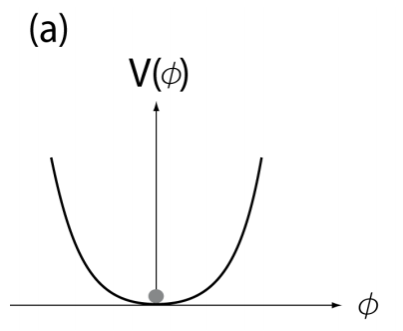
\includegraphics[scale=0.55]{Potencial Higgs.png}
        \caption\tiny{{Forma del potencial para $\mu_i^2>0$}}  
    \end{center}
\end{figure}


   \item\underline{ \textbf{Si \( \mu_\Phi^2> 0 \):}} El valor del potencial es cero, en teoría cuántica de campos es un valor esperado del campo en el vacío nulo, el cual es simétrico bajo el grupo \(SU(2)_L \otimes U(1)_X\) y se expresa de la siguiente manera: 
    
\[\fbox{$\langle  \phi \rangle_0= \langle  \triangle \rangle_0= 0$}\] 

\begin{figure}[h!]
    \begin{center}
        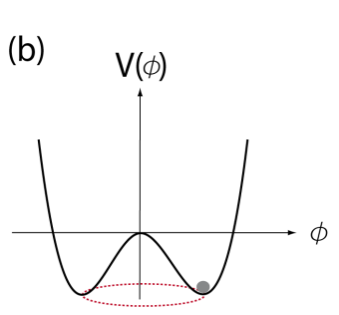
\includegraphics[scale=0.55]{Higgs Potential.png}
        \caption\tiny{Forma del potencial para $\mu_i^2\leq 0$}  
    \end{center}
\end{figure}
\end{itemize}

De esta manera, se puede expresar el potencial en términos de campos con el valor esperado en el vacío igual a cero (vacío de partículas), es decir que los campos pueden ser escritos como: 


\begin{equation}
    \Phi=\hat\Phi+ \langle \hat\Phi \rangle_0 = \begin{aligned}
   = \binom{\phi^{+}}{\frac{1}{\sqrt{2}}(v_\phi+ H + i\varsigma) } \\ 
\end{aligned}
\end{equation}

Con un valor esperado de vacío

\begin{equation}
    \langle \hat\Phi \rangle_0= \begin{aligned}
   \frac{1}{\sqrt{2}} \binom{0}{v_\phi } \\ 
\end{aligned}
\end{equation}

y para el triplete escalar: 



\begin{equation}
\triangle=\hat\triangle+ \langle \hat\triangle \rangle_0 =
\begin{aligned}
    \begin{pmatrix}  \triangle^{++} \\ \triangle^+ \\  v_\triangle+ \triangle^0 \end{pmatrix} \\
\end{aligned}
\end{equation} \\

Con un respectivo valor esperado de vacío dado por:

\begin{equation}
\langle \hat\triangle \rangle_0 =
\begin{aligned}
    \begin{pmatrix}  0 \\ 0 \\  v_\triangle \end{pmatrix} \\
\end{aligned}
\end{equation} \\
 
 
Donde, se ha tenido en cuenta que el escalar neutro se puede escribir de la siguiente manera:

\[\triangle^{0}=\frac{1}{\sqrt{2}}(R_{\triangle^{0}}^{2} + iI_{\triangle^{0}}^{2} )\]

Con su respectiva componente $\triangle^{0*}$:

\[\triangle^{0*}=\frac{1}{\sqrt{2}}(R_{\triangle^{0}}^{2} - iI_{\triangle^{0}}^{2} )\] \\

Para hallar los valores que toman los coeficientes $\mu^{2}_\Phi$ y $M^{2}_\triangle$ en los potenciales $V(\Phi,\triangle)$, del triplete añadido y del doblete escalar de Higgs del modelo estándar se aplica la condición del mínimo: 


\begin{equation}
    \frac{\partial{\langle V(\Phi, \triangle) }\rangle }{\partial v_\triangle} = \frac{\partial{\langle V(\Phi,\triangle) }\rangle }{\partial v_\phi}= 0
\end{equation}\\ 

Como se puede observar, se analiza el potencial como una función del escalar VEVs (Valor esperado de vacío). Con  $v_\phi \equiv \langle \Phi \rangle$,  $v_\triangle \equiv \langle \triangle \rangle$. Por lo tanto, podemos reescribir  el potencial mostrado en la ecuación (\ref{eq:POtencialMAjorana1})  en términos de los  VEVs

  \begin{equation}
  \begin{aligned}
  \label{eq:PotencialDiracSee3}
          \langle V(\Phi, \triangle) \rangle \subseteq    \mu_\Phi^2 {v_\phi^2} + M_\triangle^2  {v_\triangle^2} + \lambda_\Phi \frac{v_\phi^4}{2} + \lambda_\triangle \frac{v_\triangle^4}{2} +  \lambda_{ \Phi-\triangle} v^2_\triangle v^2 _\phi + \rho(v_\triangle v^2_\phi) + \text{h.c} 
  \end{aligned}
    \end{equation}


Esto implica directamente que: 

\begin{itemize}
    \item $v^{2}_\phi \equiv \langle \Phi^\dagger\Phi \rangle$
    \item $v^{2}_\triangle \equiv \langle \triangle^\dagger\triangle \rangle$
\end{itemize}

Por lo tanto, aplicando las condiciones del mínimo llegamos a: 

\begin{equation}
\label{eq:primeraderivate1}
    \frac{\partial{\langle V(\Phi, \triangle) }\rangle }{\partial v_\phi} =  2\mu^{2}_\Phi v_\phi + 2\lambda_\Phi v^{3}_\phi + 2 \lambda_{\Phi-\triangle} v_\phi v^{2}_\triangle +2\rho v_\phi v_\triangle  = 0 
\end{equation}


\begin{equation}
\label{eq:primeraderiv1}
      v_\phi(\mu^{2}_\Phi  + \lambda_\Phi v^{2}_\phi +  \lambda_{\Phi-\triangle} v^{2}_\triangle +\rho v_\triangle)  = 0
\end{equation} \\



\begin{equation}
\label{eq:primeraderivate2}
    \frac{\partial{\langle V(\Phi, \triangle) }\rangle }{\partial v_\triangle} =  2M^{2}_\triangle v_\triangle + 2\lambda_\triangle v^{3}_\triangle + 2v_\triangle \lambda_{\Phi-\triangle} v^{2}_\Phi + \rho v^{2}_\Phi = 0 
\end{equation}


\begin{equation}
\label{eq:primeradee2}
   v_\triangle( M^{2}_\triangle  + \lambda_\triangle v^{2}_\triangle +  \lambda_{\Phi-\triangle} v^{2}_\Phi) + \frac{1}{2}\rho v^{2}_\Phi = 0
\end{equation} \\

De las condiciones (\ref{eq:primeraderiv1}) y (\ref{eq:primeradee2})  se obtiene directamente las dos soluciones para los parámetros $ \mu_\triangle^2$ y $M_\Phi^2 $ con $v_\phi \neq 0 $:  \\


\begin{equation}
\begin{aligned}
\label{eq:solutionmu1}
\mu^{2}_\Phi = \lambda_\Phi v^{2}_\phi +  \lambda_{\Phi-\triangle} v^{2}_\triangle +\rho v_\triangle \\
M^{2}_\triangle = -(\lambda_\triangle v^{2}_\triangle +  \lambda_{\Phi-\triangle} v^{2}_\Phi) - \frac{\rho v^{2}_\Phi}{ v_\triangle} \end{aligned}
\end{equation} \\


Donde se ha asumido que $M^{2}_\triangle>0$ , $\mu^{2}_\Phi<0$ y $\lambda_{\triangle }$ , $\lambda_{\Phi }$ ,$ \lambda_{\Phi- \triangle} >0 $. Además teniendo en cuenta que la masa física se puede definir de la siguiente manera:

\[M^{2}_\triangle =  \mu^{2}_\triangle + v(\text{vevs}) \]

Donde, 

\begin{itemize}
\item $v(\text{vevs}) \rightarrow $  Contribución que proviene de los valores esperados de vacío (vevs)

\item $ \mu^{2}_\triangle \rightarrow  $ Parámetro en el potencial
\end{itemize}

Tomando,

\[M^{2}_\triangle \gg v(\text{vevs}) \]



donde se define, $ v(\text{vevs}) = v_\Phi$
Por lo tanto, 

\begin{equation}
    \label{eq:relation2}
M^{2}_\triangle \gg v_\Phi\end{equation}

Lo que implica que: 


 \begin{equation}
     \label{eq:RElation}
     M^{2}_\triangle \gg v^{2}_\Phi
 \end{equation}

Además teniendo en cuenta que:

\begin{equation}
    \label{eq:relation}
    v_\Phi \gg v_\triangle
\end{equation}

Reemplazando la relación (\ref{eq:relation}) y teniendo en cuenta que $M^{2}_\triangle>0$ en las ecuaciones (\ref{eq:solutionmu1}) se obtiene: 

\begin{equation}
   \label{eq:M1}
   \mu^{2}_\Phi \approx  \lambda_{\Phi} v^{2}_\Phi 
\end{equation}

Teniendo en cuenta la relación (\ref{eq:RElation}) en la ecuación (\ref{eq:primeradee2})  tenemos:

\begin{equation}
\label{eq:pri2}
   v_\triangle M^{2}_\triangle   + \frac{1}{2}\rho v^{2}_\Phi = 0
\end{equation} \\

Por lo tanto, el valor esperado de vacío del triplete escalar pesado de Higgs se puede expresar como:

\begin{equation}
    \label{eq:valoresperadodevacío}
     v_\triangle = - \frac{\rho v^{2}_\phi}{M^{2}_\triangle}
\end{equation}

%-------------------------------------------------------------------

\subsection{El lagrangiano de Yukawa:} 

Describe el acoplamiento entre el campo de Higgs y los fermiones. Por medio de una ruptura espontánea de la simetría, los fermiones adquieren una masa proporcional al valor esperado en el vacío del campo de Higgs. 

Según la ecuación (\ref{eq:21}) el lagrangiano de Yukawa tiene términos bilineales, donde no se toma en consideración la tercera ecuación de (\ref{eq:21}), debido a que se descarta la forma de singlete, así el lagrangiano más general tiene la siguiente muy forma: 

\begin{equation}
    \label{eq:51}
    \mathcal{L}_Y=  \sum_{n,m=1}^3 [ h^{nm} \overline{\psi^{ni}}_L ({\psi_R^{m}})\phi^i + \frac{1}{\sqrt{2}} Y^{nm} \overline{\psi_L^{ni}} ({\psi_L^{mj}})^{c} \triangle^{ij}] + h.c
\end{equation}

Donde, 

\begin{itemize}
    \item $Y^{nm}$ y $h^{nm} \rightarrow $ constantes de acoplamiento. 
\end{itemize}

  

Luego, del Lagrangiano expresado en la ecuación (\ref{eq:51}) se obtiene que: \\

\begin{equation}
    \mathcal{L}_Y= \frac{1}{\sqrt{2}} \sum_{n,m=1}^3 Y^{nm} \overline{\psi_L^{ni}} ({\psi_L^{mj}})^{c} \triangle^{ij} + h.c 
    \label{eq:17}
\end{equation}  \\

Considerando solo términos de masa y acoplamiento leptón - leptón.
Observamos que como consecuencia de la introducción del triplete escalar, es decir del triplete del bosón de Higgs los neutrinos adquieren masa, lo cual puede ser expresado como:\\


\begin{equation}
    \label{eq:mass5}
\begin{aligned}
\mathcal{L}^\triangle_{l-l}= \frac{v_\triangle}{\sqrt2} [Y^{11}\overline{\nu}_{e_L}({\nu}_{e_L})^c + 2Y^{12}\overline{\nu}_{e_L}({\nu}_{\mu_L})^c+ 2Y^{13}\overline{\nu}_{e_L}({\nu}_{\tau_L})^c+ \\
Y^{22}\overline{\nu}_{\mu_L}({\nu}_{\mu_L})^c + 2Y^{23}\overline{\nu}_{\mu_L}({\nu}_{\tau_L})^c+ Y^{33}\overline{\nu}_{\tau_L}({\nu}_{\tau_L})^c
]
\end{aligned}
\end{equation} \\

En este caso sólo se considera el acoplamiento ente leptones y no se tiene en cuenta los términos de interacción leptón-leptón-$\triangle$. 

De la ecuación (\ref{eq:mass5}) se genera la siguiente estructura general del lagrangiano de masa para los neutrinos

\begin{equation*}
    \mathcal{L}^\nu_{\text{masa}}= \frac{v_\triangle}{\sqrt{2}} (\begin{array}{ccc}
         \overline{\nu}_{e_L} & \overline{\nu}_{\mu_L} & \overline{\nu}_{\tau_L} )\begin{pmatrix}    Y^{11} &  Y^{12} & Y^{13} \\
         Y^{21} &  Y^{22} & Y^{23}  \\
         Y^{31} &  Y^{32} & Y^{33}  \end{pmatrix}
  \begin{pmatrix}
         (\nu_{e_L})^c \\
         (\nu_{\mu_L})^c \\
         (\nu_{\mu_L})^c 
    \end{pmatrix}
    \end{array}
    \label{eq:mass1}
\end{equation*} 

Observamos consecuentemente que como consecuencia de la introducción del triplete escalar, los neutrinos adquieren masa, es decir el lagrangiano anterior puede ser expresado como:  

\begin{equation}
    \mathcal{L}^\nu_{\text{masa}}= \frac{1}{2} (\begin{array}{ccc}
         \overline{\nu}_{e_L} & \overline{\nu}_{\mu_L} & \overline{\nu}_{\tau_L} )M_{mn}    \begin{pmatrix}
         (\nu_{e_L})^c \\
         (\nu_{\mu_L})^c \\
         (\nu_{\mu_L})^c 
    \end{pmatrix}
    \end{array}
    \label{eq:mss2}
\end{equation} 

Donde, la matriz de masa \(M_{mn} \) está definida de la siguiente manera: 

\[M_{mn} = \sqrt{2}v_\triangle Y^{mn}\] 

Las masas de los neutrinos que hemos obtenido con este mecanismo
es proporcional al valor esperado de vacío del triplete escalar pesado de Higgs  $v_\triangle  $, en forma similar a como se generan
las masas de los quarks y leptones cargados. Sin embargo, es conocido
que las masas de los neutrinos son mucho más pequeñas que la de los
quarks y leptones cargados. \\

\begin{equation}
    M_{mn} = \sqrt{2}v_\triangle \begin{pmatrix}    Y^{11} &  Y^{12} & Y^{13} \\
         Y^{21} &  Y^{22} & Y^{23}  \\
         Y^{31} &  Y^{32} & Y^{33}  \end{pmatrix}
       \label{eq:20}  
\end{equation} \\

\begin{itemize}
    \item \(v_\triangle \rightarrow  \) toma valores muy pequeños
en comparación con el valor esperado de vacío del doblete escalar $v_\phi$ debido a que la masas del triplete de Higgs es grande
\end{itemize}
\[v_\triangle \ll v_\phi \]
  
Teniendo en cuenta que el valor esperado de vacío del triplete escalar de Higgs añadido puede expresarse como

\begin{equation}
    \label{eq:valoeradodevacío}
     v_\triangle = - \frac{\rho v^{2}_\phi}{M^{2}_\triangle}
\end{equation}

De está manera, podemos escribir la ecuación (\ref{eq:20}) de la siguiente manera: \\

\begin{equation}
    M_{mn}= -\frac{\sqrt{2}\rho v^{2}_\phi Y^{mn}}{M^{2}_\triangle} 
\end{equation} \\

Introduciendo un valor de masa grande para el término de \( M^{2}_\triangle \) se obtiene un valor liviano para las masas de los neutrinos \( M_{mn} \); por lo tanto se concluye que el \textbf{mecanismo Seesaw tipo II} genera neutrinos ligeros mediante la introducción de Higgs pesados. \\

Pasamos a los estados de masa mediante la diagonalización de la
matriz \( M_{mn} \), esto bajo la ecuación: 
\begin{equation}
   UM_\nu U^\dagger= M_{mn}
\label{eq:23}
\end{equation}

\begin{itemize}
\item \( U \rightarrow \) matriz de Pontecorvo-Maki-NakagawaSakata. La cual viene descrita de la siguiente manera:

\begin{equation}
        U =  \begin{pmatrix}    c_{12}c_{13} & s_{12}c_{13} & s_{13}e^{-i\delta} \\
         -c_{23}s_{12}-s_{13}s_{23}c_{12}e^{i\delta} &  c_{23}s_{12}-s_{13}s_{23}s_{12}e^{i\delta} & s_{23}c_{13}  \\
         s_{23}s_{12}-s_{13}c_{23}c_{12}e^{i\delta} &  -s_{23}c_{12}-s_{13}c_{23}s_{12}e^{i\delta} & c_{23}c_{13}  \end{pmatrix} \begin{pmatrix}   1 & 0 & 0 \\
         0 &  e^{i\varphi_1} & 0  \\
        0 &  0 & e^{i\varphi_2}  \end{pmatrix}
       \label{eq:24}  
\end{equation} \\

\item \( s_{ij}\) y \(c_{ij} \rightarrow \) \( \sin\theta_{ij}  \) y \( \cos\theta_{ij}  \) respectivamente. 
\item \(\delta \rightarrow \)  son ángulos de mezcla y la fase de
Dirac que en principio se pueden caracterizar en experimentos de oscilación de neutrinos.

\item \(\varphi_1 \) y \(\varphi_2 \) fases adicionales por la naturaleza de Majorana de los neutrinos. 

\end{itemize}

Obteniendo finalmente que: 
 
\begin{equation}
    M_\nu=  \begin{pmatrix} m_1& 0 & 0  \\ 0 & m_2 & 0 \\ 0 &0 & m_3   \end{pmatrix} 
\end{equation} 

Donde \( m_1 \),\( m_2 \) y \( m_3 \) son las masas físcas para los tres neutrinos. 


De las ecuaciones (\ref{eq:20}) y (\ref{eq:23})  se obtiene la relación que acopla las constantes de Yukawa y los parámetros medidos en experimentos de oscilación de neutrinos. 

\begin{equation}
Y^{nm}=\frac{UM_{\nu}U^{T}}{\sqrt{2}v_\triangle}
    \label{eq:26}
\end{equation}


\begin{figure}[h!]
  \begin{center}
  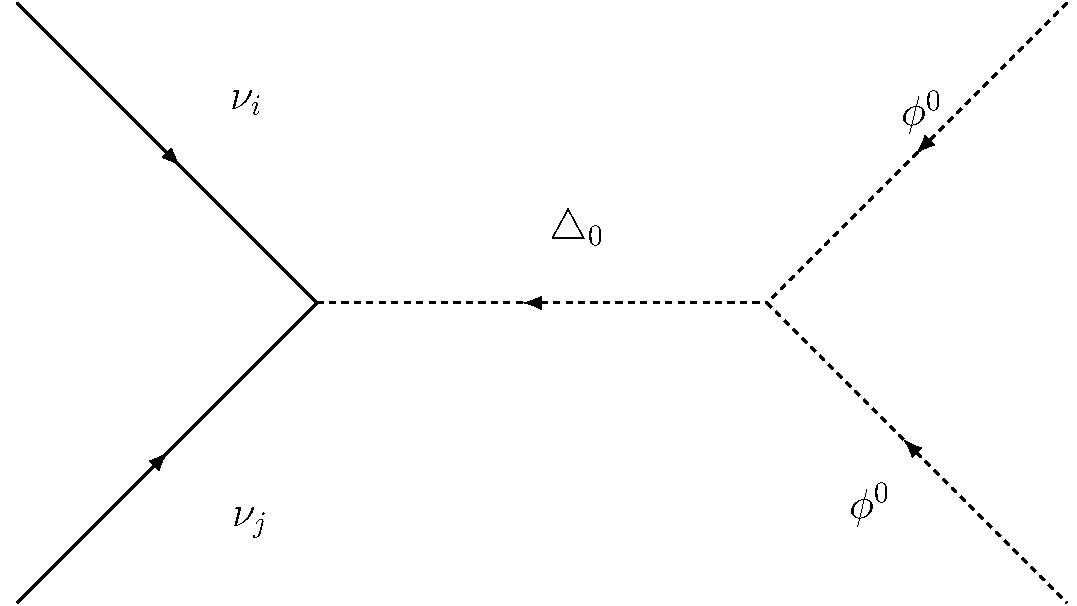
\includegraphics[scale=0.4]{Mecanismo See-saw tipo IIMajorana.pdf}
\caption{{\textbf{Mecanismo Seesaw tipo II}: Interacción de los campos mediante el intercambio de campo escalar.}}
\label{fig:Majorana2}
\end{center}
\end{figure}

En este mecanismo la interacción de campos intercambiando un triplete escalar de Higgs (ver figura \ref{fig:Majorana2}) genera un vértice efectivo, por lo que la constante de acoplamiento
efectiva se expresa como: 

\begin{equation}
    \kappa_\triangle=\frac{\rho Y^{nm}}{M^{2}_\triangle }
\end{equation}

Por lo tanto, se puede concluir que a bajas energías se pueden obtener los mecanismos Seesaw tipo I y II mediante operadores efectivos, por lo que no nos permite diferenciar un mecanismo de otro en estas energías.


%-----------------------------------------------------------------------
\section{Mecanismo Seesaw tipo II- Masas de Dirac}

Se propone un modelo de Dirac seesaw tipo II para obtener las pequeñas masas de neutrinos extendiendo el contenido visible del modelo estándar (SM) con un sector oculto compuesto por un singlete escalar $S$ y tres  neutrinos singletes derechos $(\nu_{R_1},\nu_{R_2}, \nu_{R_3} )$. Estos neutrinos singletes derechos se cargan bajo una nueva simetría $U(1)_{B-L}$. Además es necesario añadir dos dobletes escalares pesados para desempeñar el rol de mensajero entre el sector visible (SM) y el sector invisible (neutrinos singletes derechos y singlete). 





\subsection{Simetrías $U(1)_{B-L}$ } 
%MEJORAR PUEDE DAR MÁS 

Al extender el contenido visible del modelo estándar con un sector oculto, el cual se prescribe mediante una simetría gauge abeliana local $U(1)_{B-L}$ automáticamente aparecen anomalías en el modelo. Esto implica que las anomalías en las simetrías gauge matan a toda la física por completo: ¡hacen que la teoría sea matemáticamente inconsistente!. Esto se debe a que cuando introducimos un fermión de una sola helicidad (derecha o izquierda) la teoría cuántica de campos se descompensa. Si deseamos construir una teoría consistente, entonces debemos asegurarnos de que todas las anomalías desaparezcan. \\ 


El modelo estándar (SM) de quarks y leptones está libre de anomalías gauge. En nuestro  caso la simetría gauge local añadida al SM consiste en tres  neutrinos singletes derechos $(\nu_{R_1},\nu_{R_2}, \nu_{R_3} )$ y un singlete escalar $S$, las condiciones para la ausencia de anomalías de gauge imponen restricciones no triviales. \\ 




\subsubsection{Cancelación de anomalías}

Las soluciones a las condiciones de cancelación de anomalías nos permiten escribir las cargas $B-L$ de los campos del modelo estándar de la siguiente manera:  

\begin{equation}
 X (r,l)=rR-lY   
\end{equation} \\

Donde, $R$ es el generador de $U(1)_R$, $Y $ es la hipercarga, $l$ es la carga $X$ del doblete leptónico, en nuestro caso se considera, $X={B-L}$ y $r$ parametriza la contribución a las anomalías gravitacionales. \\

Al SM se le está añadiendo una simetría nueva abeliana local, que tiene carga nueva ${B-L}$. Por lo que todo lo que satisface la hipercarga ${Y}$ para la simetría $U(1)_Y$ lo debe satisfacer está nueva carga. Cuando se introduce una simetría arbitraria con carga nueva ${B-L}$ entonces lo que se debe garantizar es que los fermiones de Weyl nuevos que se añadan tienen que garantizar la siguiente ecuación \cite{Restrepo}:


\begin{equation}
\label{eq:triplet}
    \sum_{\alpha=1}^N n'_{\alpha}=-3 
\end{equation}

\begin{equation}
\label{eq:triplet1}
    \sum_{\alpha=1}^N n'^{3}_{\alpha}=-3 
\end{equation}

Las ecuaciones (\ref{eq:triplet}) y (\ref{eq:triplet1}) hacen referencia a la suma de las cargas nuevas de los fermiones de Weyl izquierdos añadidos. Donde, $N$ número de fermiones añadidos. \\ 

La cancelación de anomalías implica que se deben agregar al menos tres neutrinos derechos al contenido mínimo de representación del modelo estándar electrodébil. Sin embargo, surgen dos tipos de modelos:

\begin{enumerate}
\item Cada uno de los tres neutrinos derechos tienen un número total de leptones 
\begin{equation}
\label{eq:triplet2}
    \sum_{\alpha=1}^N U(1)_{B-L}^{3}=-3 
\end{equation}
\item En nuestro trabajo se considera uno de los casos más simples para las tres familias. Consideremos que $\nu_{R_i} \approx n_i $ bajo $U(1)_{B-L}$. Entonces $n_{1,2,3}=(-4,-4,+5)$. Podemos verificar que:


\begin{equation}
\label{eq:triplet3}
    \sum_{\alpha=1}^N n'_{\alpha}=(-4) + (-4)+ (+5) = -3
\end{equation}

Además se cumple,  

\begin{equation}
\label{eq:triplet4}
    \sum_{\alpha=1}^N n'^{3}_{\alpha}=(-4)^3 + (-4)^3+ (+5)^3 = -3
\end{equation}
\end{enumerate}.

%--------------------------------------------------------------------

\subsection{Construcción del Modelo }:


Considerando una extensión del modelo estándar (SM) basada en la siguiente simetría gauge: 

\begin{equation}
\begin{aligned}
 SU(3)_c \otimes SU(2)_L \otimes U(1)_{Y^ \text{'}} \otimes U(1)_{B-L}  \\
    \downarrow \langle S \rangle  \\
    SU(3)_c \otimes SU(2)_L \otimes U(1)_{Y} \\
     \downarrow \langle \phi \rangle  \\
     SU(3)_c \otimes  U(1)_{\text{em}}
\end{aligned}
\end{equation}\\

Donde, $Y^ \text{'} $ es elegido en orden para obtener la hipercarga, $Y$ del Modelo Estándar. Como se ha mencionado anteriormente, $\langle S \rangle $ corresponde a un singlete y $\langle \phi \rangle$ a un doblete bajo la simetría $SU(2)_L$.  \\


El contenido de campo del modelo $SU(2)_L\otimes U(1)_{Y^ \text{'}} \otimes U(1)_{B-L} $ que proponemos en este trabajo se determina en la Tabla \ref{tab:SeesawType II}. Donde $L$ representa un doblete de leptones zurdos, $\phi$ el doblete de Higgs, $\nu_R$ los neutrinos singlete derechos, $S$ el singlete Higgs y $\eta$ los dobletes escalares pesados. Debido a que las partículas del SM no se encuentran cargadas bajo la nueva simetría añadida $U(1)_{B-L}$, mientras que los neutrinos derechos sí; se prohíbe el acoplamiento de Yukawa de los dobletes leptónicos $L$ y los neutrinos singletes derechos con el doblete de Higgs ligero $\phi$. Es decir que, como se representa en la figura (\ref{fig:sectores}), el sector invisible que contiene al singlete escalar Higgs $S$ y los neutrinos derechos se encuentra oculto del sector visible del SM compuesto por el doblete de Higgs $\phi$ y un doblete leptónico $L$. Esto implica que los dobletes escalares pesados $\eta$ no solo se unen al grupo gauge $SU(2)_L \otimes U(1)_Y$ sino también al nuevo, une los dos sectores.\cite{Hong}  \\

\begin{figure}[h!]
\begin{center} 
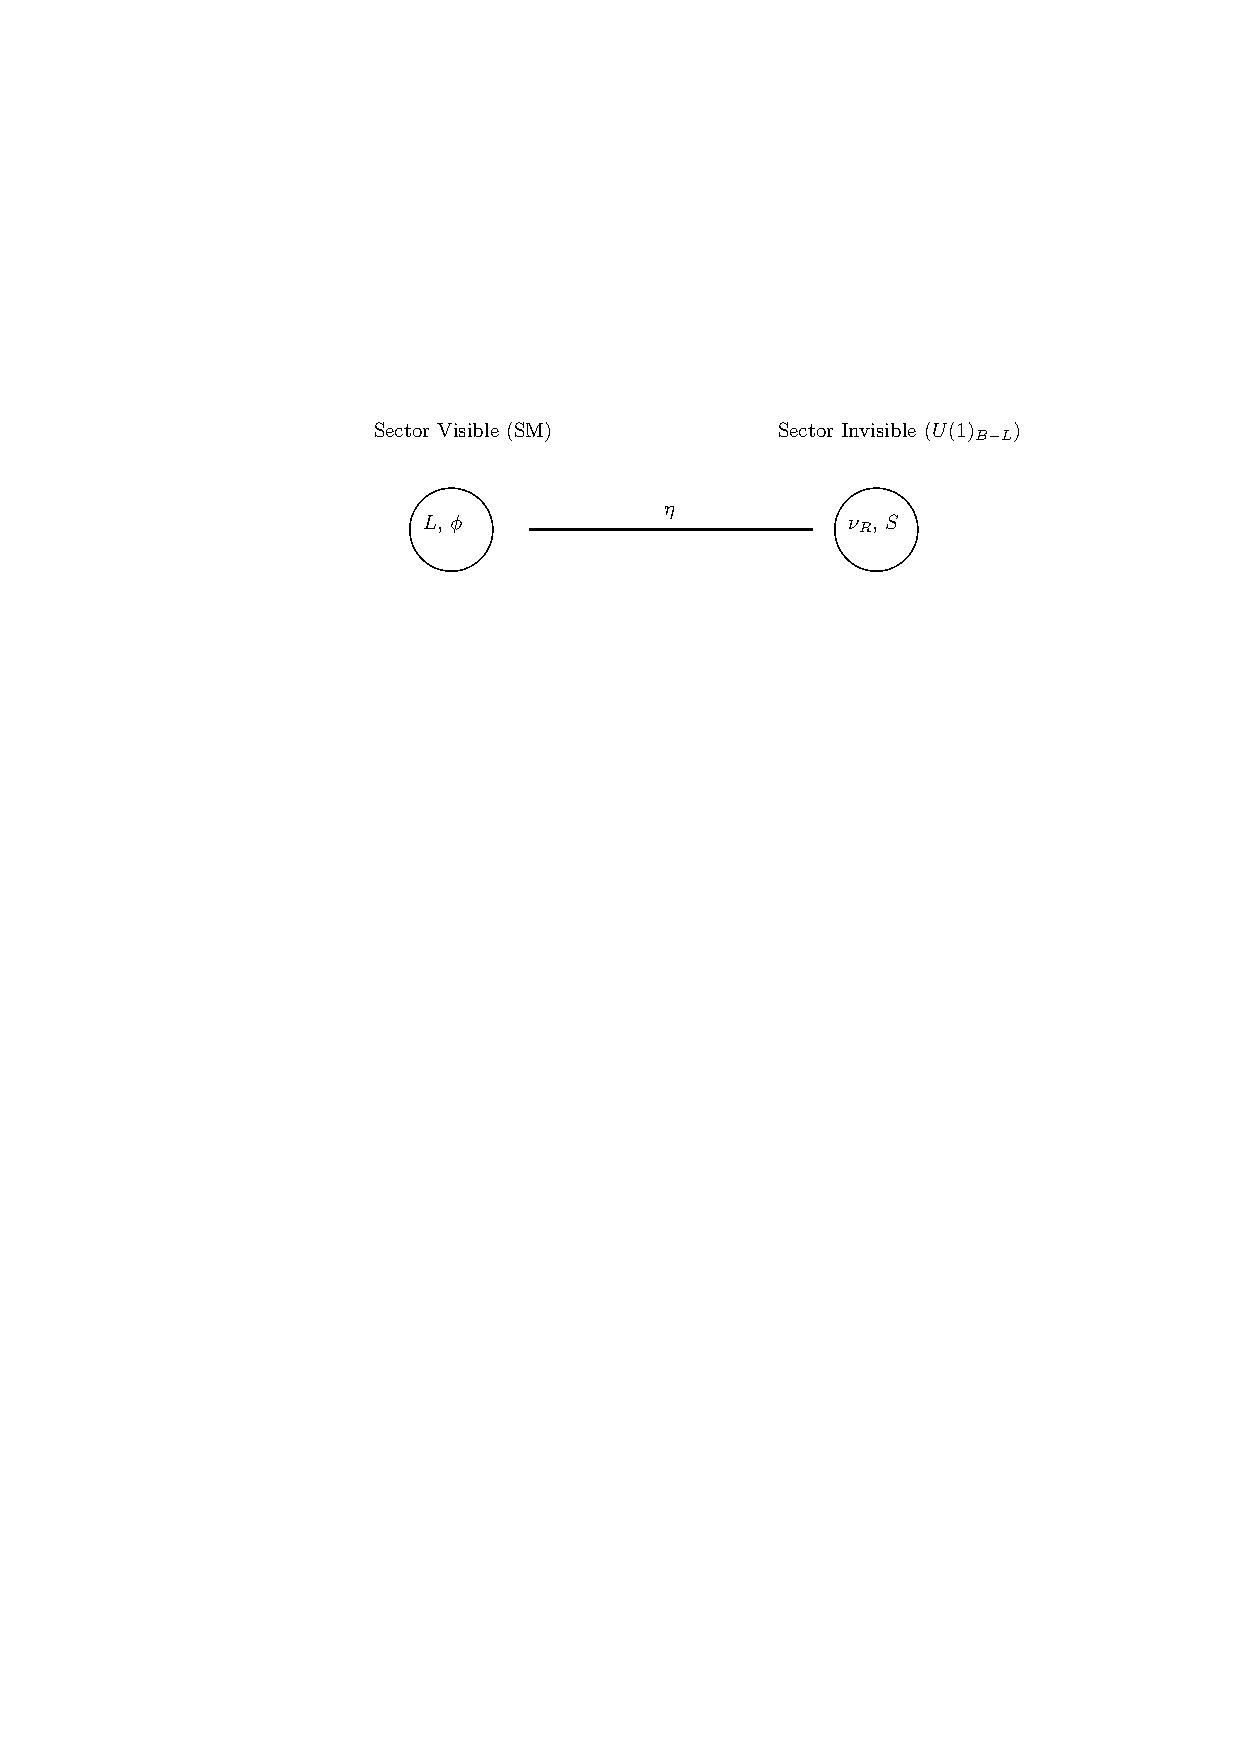
\includegraphics[scale=1.0]{sectors.pdf}
\caption{ Los dobletes escalares pesados $\eta$ actúan como mensajeros entre los sectores visibles los cuales corresponden al SM y el sector invisible.}
\label{fig:sectores}
\end{center}
\end{figure}

%%%IMPORTANTE REFERENCIAR AL PAPER Neutrino Mass and Baryon Asymmetry from Dirac Seesaw

%---------------------------------------------------------------
\subsection{Representación de Interacciones}:

Como los términos en el Lagrangiano respetan todas las cargas conservadas, podemos visualizar los términos de corrientes que fluyen %%%%CITAR LIBRO DE DIEGO CAPITULO 8
a través; en esté trabajo se tiene en cuenta el diagrama mostrado en la figura (\ref{fig:Majorana}),  donde se tienen en cuenta dos vértices, $(a)$ y $(b)$. \\

\begin{figure}[h!]
  \begin{center}
  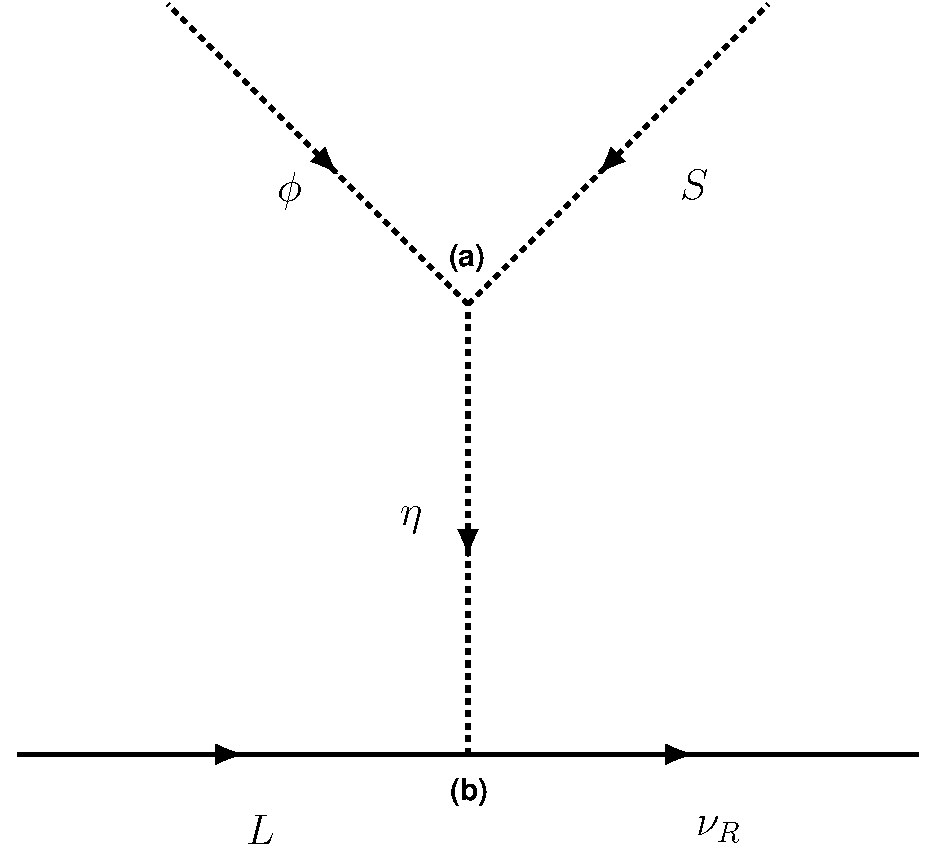
\includegraphics[scale=0.6]{DiracSeeSAWdiagram.pdf}
\caption{{\textbf{Mecanismo Seesaw tipo II}: Interacción de los campos mediante el intercambio de campo escalar.}}
\label{fig:Majorana}
\end{center}
\end{figure}

Teniendo en cuenta que L corresponde al doblete leptónico, dado por:\\ 


\begin{equation}
\begin{aligned}
    \label{eq:DobleteL}
      L & = \binom{\nu}{e}_L & :  (\textbf{2}, -1/2)  
\end{aligned}
\end{equation}\\

Por lo tanto, el doblete leptónico $L$ está dotado con una hipercarga correspondiente a $-\frac{1}{2}$. El flujo de hipercarga puede ser visualizado en la figura (\ref{fig:Hypercharge(a)}). Donde la línea punteada representa a las partículas escalares mientras que la línea continua a los fermiones. 


\begin{figure}[h!]
  \begin{center}
  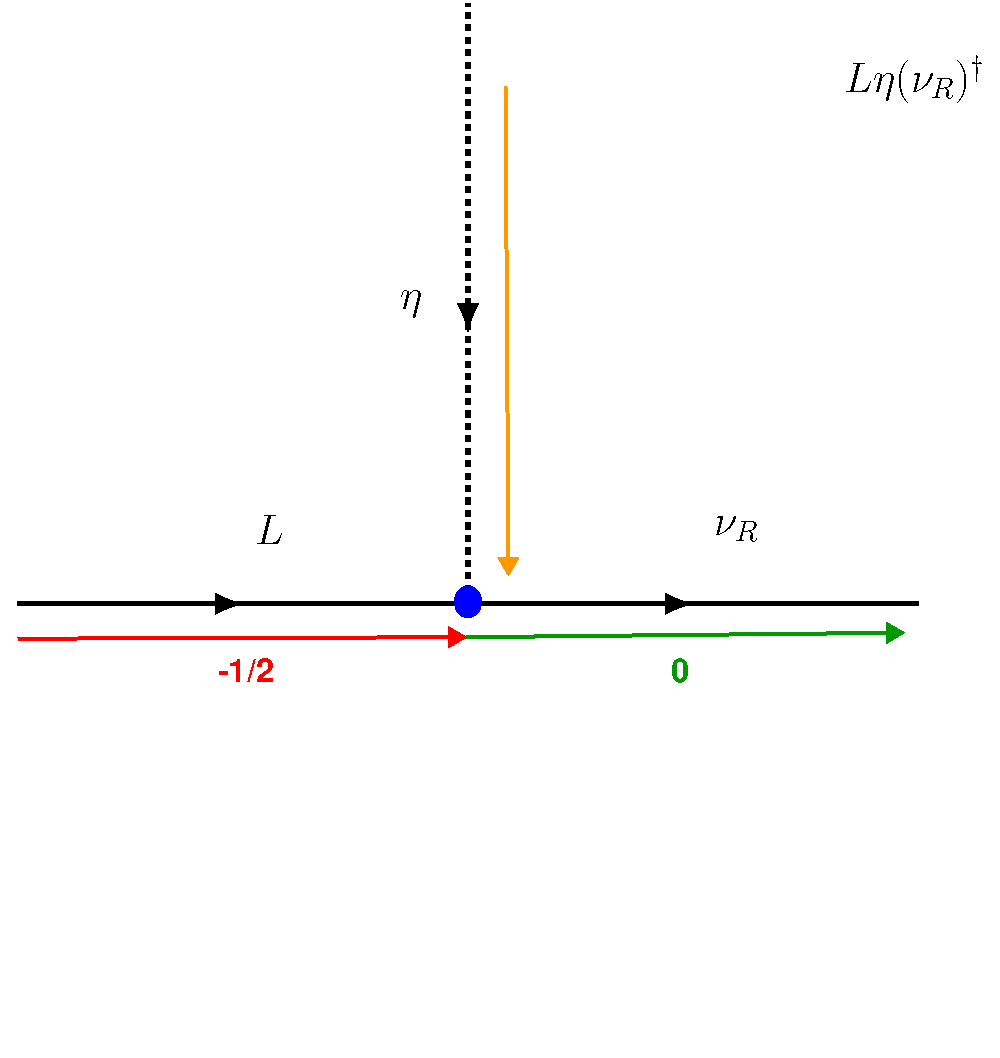
\includegraphics[scale=0.6]{Flujohyer(a).pdf}
\caption{{\textbf{Flujo de hipercarga en el vértice (b)}: Al vértice azul entra un doblete leptónico con hipercarga $\color{red}
-\frac{1}{2}$ y sale un neutrino singlete con hipercarga igual a $\color{green} 0 $, Por lo tanto se concluye que al vértice debe entrar un doblete escalar pesado $\eta$ con hipercarga igual a $ \frac{1}{2}$.}}
\label{fig:Hypercharge(a)}
\end{center}
\end{figure}

Por lo tanto, escribiendo las ecuaciones para dicho vértice, donde las cargas que entran al vértice azul se deben igualar a las que salen se obtiene que: \\

     \underline{\textbf{Ecuaciones para $U(1)_Y$}}:  
\begin{itemize}
    \item Vértice (b):
    \begin{equation}
    \label{eq:eqforhypercharge}
    \begin{aligned}
            L+\eta=\nu_R \\
            \frac{-1}{2} + \eta = 0 \\
            \fbox{$ \eta=\frac{1}{2}$}
    \end{aligned}
    \end{equation}
\end{itemize}

De está manera, se obtiene que el doblete escalar pesado $\eta$ tiene una hipercaga correspondiente a $\frac{1}{2}$. \\

 Escribiendo el término del lagrangiano con el doblete escalar pesado $\eta$, el doblete leptónico $L$ y el neutrino singlete derecho como:

\begin{equation}
    \label{eq:LaYukawa(a)}
     \mathcal{L}_{Y_{(b)}} =  y (\nu_R)^*{L}\cdot\eta
\end{equation} \\

Luego, considerando que el singlete escalar de Higgs puede ser expresado de la siguiente manera:

\begin{equation}
\begin{aligned}
 \label{eq:SingleTe1}
    S=\frac{1}{\sqrt{2}}(v_S+ R_S+iI_S) & : (\textbf{1}, 0) 
\end{aligned}
\end{equation}

Tenemos entonces que el singlete escalar de Higgs $S$ está dotado con una hipercarga correspondiente a $0$. El flujo de hipercarga puede ser visualizado en la figura (\ref{fig:Hypercharge(a)}). Donde la línea punteada representa a las partículas escalares. \\


\begin{figure}[h!]
  \begin{center}
  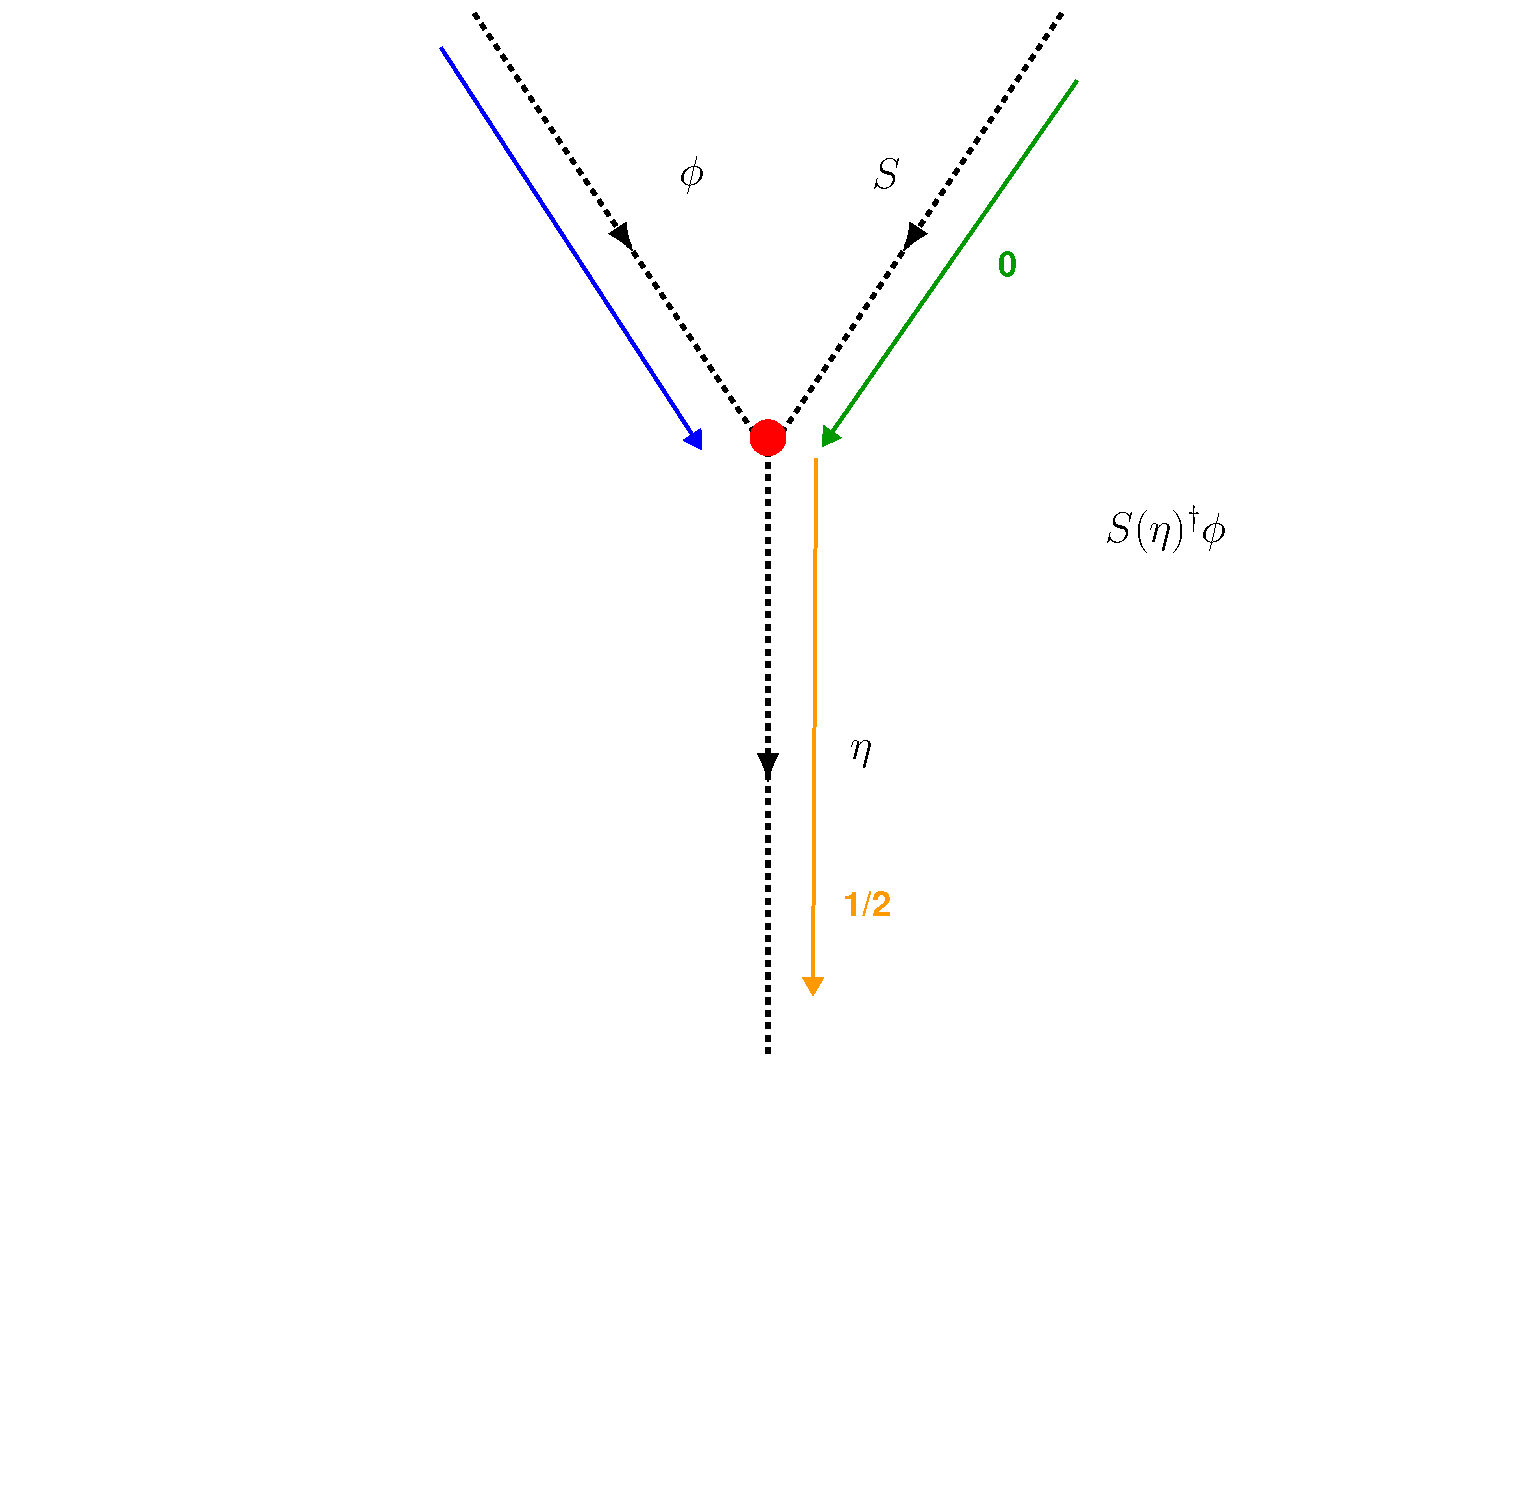
\includegraphics[scale=0.5]{Flujodriagram(b).pdf}
\caption{{\textbf{Flujo de hipercarga en el vértice (a)}: Al vértice rojo entra un singlete escalar de Higgs  con hipercarga  $\color{blue} 
0$ y sale un doblete escalar pesado con hipercarga igual a $\color{orange} \frac{1}{2}$. Por lo tanto, se concluye que entra  doblete escalar de Higgs con hipercarga igual a $ \frac{1}{2}$.}}
\label{fig:Hypercharge(b)}
\end{center}
\end{figure}

Escribiendo las ecuaciones para dicho vértice, donde las cargas que entran al vértice rojo se deben igualar a las que salen se obtiene que: \\

\begin{itemize}
    \item Vértice (a):
    \begin{equation}
    \label{eq:eqforhypercharge(b)}
    \begin{aligned}
            \phi+S=\eta \\
            \phi+ 0  = \frac{1}{2} \\
           \fbox{$ \phi=\frac{1}{2}$}
    \end{aligned}
    \end{equation}
\end{itemize}

De está manera, se obtiene que el doblete escalar de Higgs $\phi$ tiene una hipercaga correspondiente a $\frac{1}{2}$. \\

 Escribiendo el término del lagrangiano con el doblete escalar de Higgs $\phi$, el doblete escalar pesado $\eta$ y el singlete escalar $S$ como:

\begin{equation}
    \label{eq:LaYukawa(b)}
     \mathcal{L}_{Y_{(a)}} =   \rho S(\eta)^\dagger\phi 
\end{equation} \\

Análogamente, para la nueva carga $(B-L)$ se considera el número leptónico como la carga nueva, es decir que el número leptónico se vuelve una carga muy importante en este modelo, esto se debe a que paso de ser una simetría global a una local; por lo tanto, sabiendo que la carga leptónica del doblete leptónico es tomada como $-1$ y en nuestro modelo se introduce $(\nu_R)^*_i= +4 $ donde $i=1,2$, y $(\nu_R)^*_3=-5$, además en el vértice azul, el flujo de carga que sale debe ser igual al flujo de carga que entra, por lo tanto se obtienen las siguientes ecuaciones:  \\

\begin{figure}[h!]
  \begin{center}
  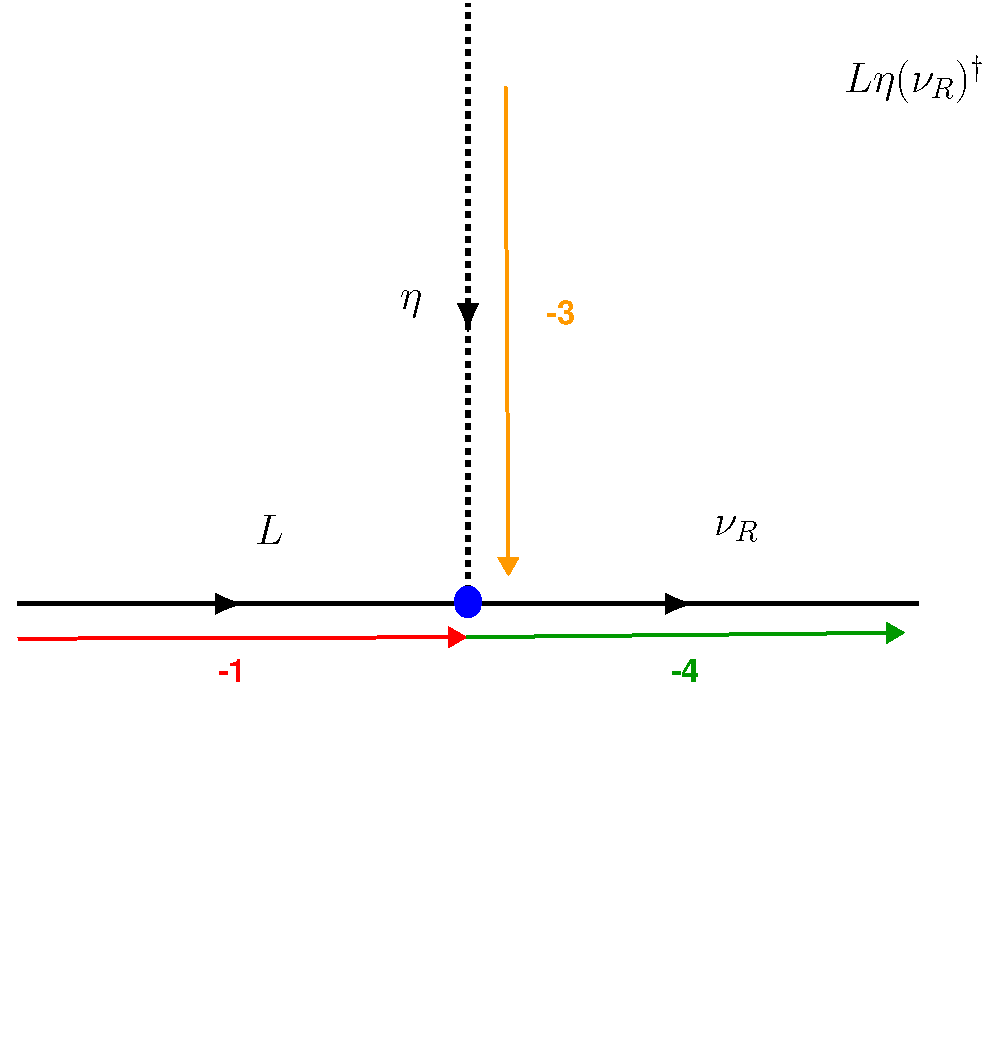
\includegraphics[scale=0.5]{DiagramB-L.pdf}
\caption{{\textbf{Flujo de carga leptónica en el vértice (b)}: Al vértice azul entra un doblete leptónico con carga leptónica igual a $-1$ y sale un neutrino singlete con carga leptónica de $-4$, Por lo tanto se concluye que al vértice debe entrar un doblete escalar pesado $\eta$ con carga leptóica igual a $ -3$. ($\color{red}-1$ $\color{orange}-3$=$\color{green}-4)
$)}}
\label{fig:B-L}
\end{center}
\end{figure}


\underline{\textbf{Ecuaciones para $U(1)_{B-L}$}}:  
\begin{itemize}
    \item Vértice (b):
    \begin{equation}
    \label{eq:eqforB-L(a)}
    \begin{aligned}
            L+\eta=\nu_R \\
            -1 + \eta =-(\nu_R)^*  \\
            \eta=-4+1  \\
            \fbox{$ \eta=-3$}
    \end{aligned}
    \end{equation}
\end{itemize} 

Por lo tanto, se concluye que el doblete escalar pesado está dotado con una carga del número leptónico $B-L$, correspondiente a $-3$. El flujo de carga del número leptónico puede ser visualizado en la figura (\ref{fig:B-L}). Donde la línea punteada representa a las partículas escalares mientras que la línea continua a los fermiones. \\



Finalmente, teniendo en cuenta que la carga del número leptónico para el doblete escalar de Higgs es $0$ y con el resultado obtenido en la ecuación (\ref{eq:eqforB-L(a)}) se puede obtener el valor de la carga del número leptónico para el singlete escalar de Higgs. El flujo de carga del número leptónico para el vértice $(a)$ ó vértice rojo, puede ser visualizado en la figura (\ref{fig:B-L(b)})


\begin{figure}[h!]
  \begin{center}
  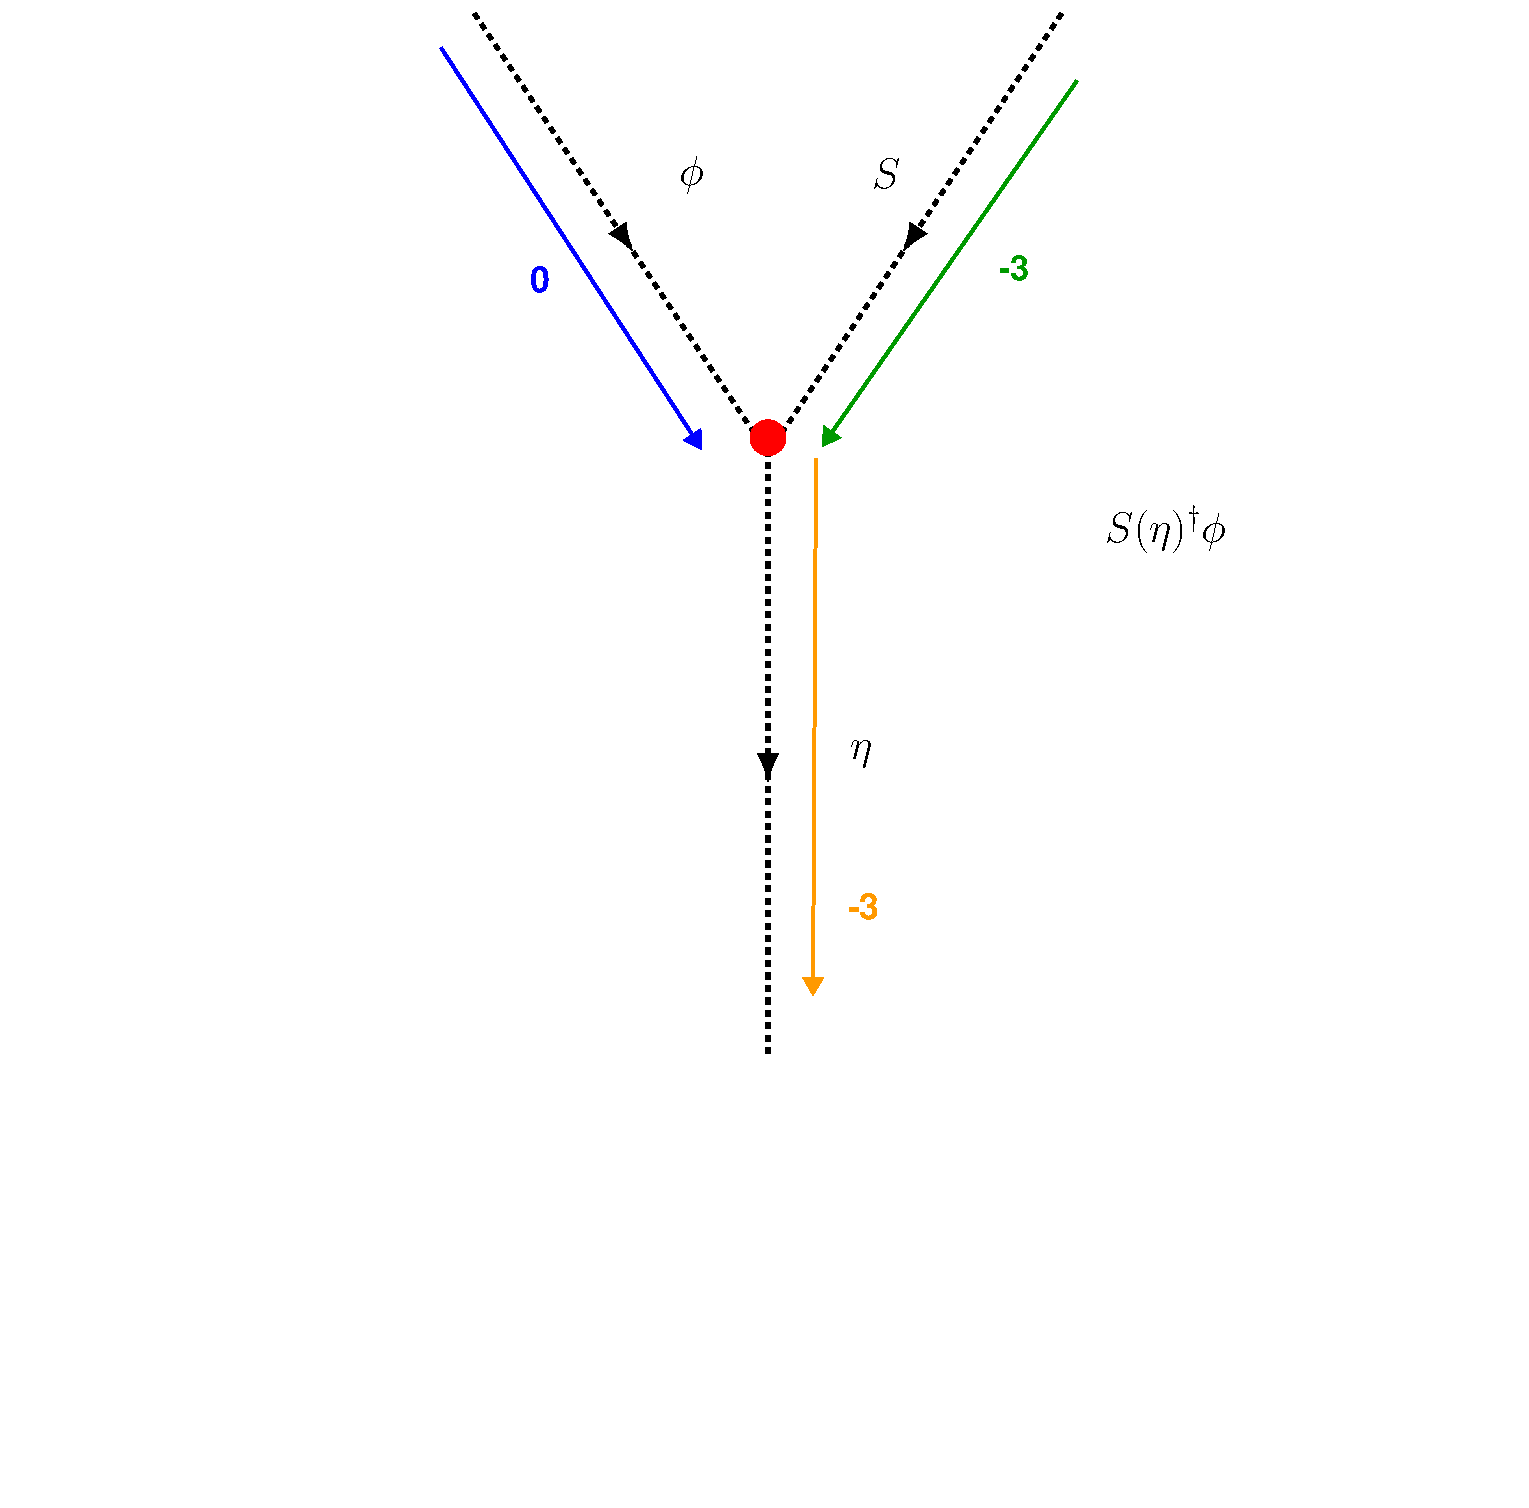
\includegraphics[scale=0.5]{Flujodriagram(b)(B_L).pdf}
\caption{{\textbf{Flujo de carga leptónica en el vértice (a)}: Al vértice rojo entra un singlete escalar de Higgs  con carga leptónica  $-3$ y un doblete escalar de Higgs con una carga leptónica correspondiente a $0$, por lo tanto,  sale un doblete escalar pesado con carga leptónica igual a $-3$. }}
\label{fig:B-L(b)}
\end{center}
\end{figure}


\begin{itemize}
    \item Vértice (a):
    \begin{equation}
    \label{eq:eqforB-L(b)}
    \begin{aligned}
            \phi+S=\eta \\
            0+ S  = -3 \\
          \fbox{$ S=-3$}
    \end{aligned}
    \end{equation}
\end{itemize}

Se concluye que el singlete escalar de Higgs se dota de una carga de número leptónico correspondiente a $-3$. \\

Finalmente, podemos completar el contenido de campo del modelo $SU(2)_L\otimes U(1)_Y \otimes U(1)_{B-L} $ con las operaciones realizadas en las ecuaciones anteriores. El cual se muestra en la Tabla (\ref{tab:SeesawType II}).


\renewcommand{\arraystretch}{2.0}
\begin{table}[h!]
\begin{center}
\begin{tabular}{| c | c | c | c | }
\hline
\multicolumn{4}{ |c| }{\textbf{Modelo $SU(2)_L\otimes U(1)_Y \otimes U(1)_{B-L} $}} \\ \hline
\textbf{Campos} & \textbf{$SU(2)_L$}  &   \textbf{$U(1)_Y$} & \textbf{$U(1)_{B-L}$} \\ \hline
$(\nu_R)^*_{i} $ & $\textbf{1}$ & $0$ &  $+4$ \\
$(\nu_R)^*_{3} $ & $\textbf{1}$ & $0$ &  $-5$ \\
$ L^{(n)} $ &  $\textbf{2}$ & $-1/2$ & $-1$ \\
$ \eta $  & $\textbf{1}$ &  $1/2$  & $-3$ \\
$ S $ & $\textbf{2}$ & $0$  &  $-3$ \\ 
$ \phi $ & \textbf{2} &  $1/2 $   & $0$ \\ \hline
\end{tabular}
\caption{El contenido de campo relacionado con la generación de las masas de neutrinos de Dirac. Donde $i=1,2$ y $L = \binom{\nu}{e}_L$}
\label{tab:SeesawType II}
\end{center}
\end{table}

%------------------------------------------------------------

\subsection{Lagrangiano de Yukawa}

Describe el acoplamiento entre los campos escalares de la teoría y los fermiones. En nuestro caso, el acoplamiento involucra a al doblete escalar pesado $\eta$, el doblete de Higgs, tipo SM $\phi$ y el escalar singlete $S$. Por medio de una ruptura espontánea de la simetría, los fermiones adquieren una masa proporcional al valor esperado en el vacío del campo de Higgs. \\

Considerando los términos del lagrangiano descritas en las ecuaciones (\ref{eq:LaYukawa(a)}) y (\ref{eq:LaYukawa(b)}), podemos escribir la interacción del lagrangiano para generar las masas de neutrinos de Dirac, además el diagrama a nivel árbol que representa dicha interacción descrita por el lagrangiano se muestra en la figura (\ref{fig:FinallyDiagram})

%Weyl
\begin{equation}
    \label{eq:Yukawasumainteractions}
    \mathcal{L}_Y \supset  -y (\nu_R)^* {L}\cdot \eta + \rho S\eta^\dagger\phi + \text{h.c}
\end{equation}
%Weyl Alternativo

Donde, 

\begin{align}
    \label{eq:cot}
    A\cdot B=&\epsilon_{ab}A^a B^b =\widetilde{A}^\dagger B
\end{align}

Por lo tanto, podemos escribir el lagrangiano de la ecuación  (\ref{eq:Yukawasumainteractions}) como:

\begin{equation}
    \label{eq:Weilalternativo}
    \mathcal{L}_Y \supset  -y (\nu_R)^* \widetilde{\eta}^\dagger {L}+ \rho S\eta^\dagger\phi + \text{h.c}
\end{equation} \\

Donde, $y \rightarrow $ Acoplamiento de Yukawa. 

El diagrama a nivel árbol para la generación de masas de neutrinos en \textbf{Mecanismo Seesaw Dirac tipo II} se muestra a continuación 

\begin{figure}[h!]
\begin{center}
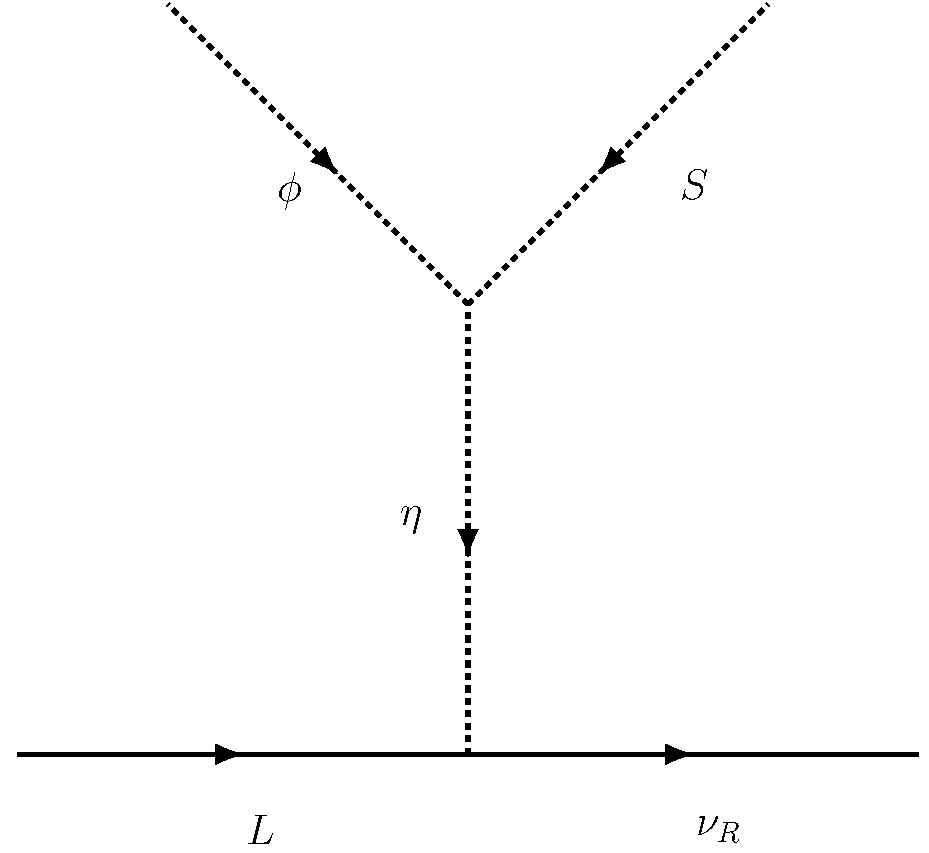
\includegraphics[scale=0.5]{DiracSeeSAWFinally.pdf}
\caption{Generación de masa de neutrinos en el mecanismo Seesaw Dirac tipo II.}
\label{fig:FinallyDiagram}
\end{center}
\end{figure}

%---------------------------------------------------------------------

\subsection{Lagrangiano de Higgs}

Teniendo en cuenta que la teoría al ser renormalizable, implica que la densidad lagrangiana no posee explícitamente términos de masa para los fermiones, ni para los bosones intermediarios ya que de lo contrario estos romperían explícitamente la simetría y harían a la teoría no renormalizable.$^{[6]}$ Por consiguiente, es necesario dotar de masa a las partículas del SM, para lo cual es necesario implementar el mecanismo de ruptura espontánea de la simetría.

Este mecanismo consiste en introducir un nuevo campo $\phi $ el cual interactúa con los bosones gauge $W^{\pm}_\mu$, $Z_\mu$ y $A_\mu$. \\

En nuestro caso, se introducen tres campos escalares,un doblete pesado $\nu$, el doblete escalar de higgs $\eta$ y un singlete $S$. Por lo tanto, el lagrangiano de  Higgs toma la siguiente forma: 

\begin{equation}
    \mathcal{L}_{\text{Higgs}}= (D_\mu\phi)^\dagger(D^\mu\phi)+ (D_\mu\eta)^\dagger(D^\mu\eta) + (D_\mu S)^\dagger(D^\mu S) + V_H
    \label{eq:HiggsDirac}
\end{equation}\\

 Se debe tener en cuenta que en está parte del trabajo se considera el caso de representaciones con dos dobletes (el doblete de Higgs, $\phi$  y el doblete pesado agregado, $\eta$) y un singlete  \(S\), en $\Phi$
 
La derivada covariante permite escribir el acople de los bosones de gauge
con los escalares \(\phi\), $\eta$ y $ S $



Por lo tanto, el potencial escalar puede ser escrito de la siguiente manera: 

    \begin{equation}
         V_H = V(\phi, S, \eta) \subseteq  \mu_\phi^2\phi^\dagger\phi +  \mu_S^2 S^* S+ M_\eta^2\eta^\dagger\eta + \lambda_\phi(\phi^\dagger\phi)^2+ \lambda_S(S^* S)^2 +     
    \end{equation}
\[ \lambda_\eta(\eta^\dagger\eta)^2 + 
     \lambda_{\phi-S}(\phi^\dagger\phi)(S^* S)+ \lambda_{\phi-\eta}(\phi^\dagger\phi)(\eta^\dagger\eta)+    \lambda_{\eta-S}(S^* S)(\eta^\dagger\eta)+  \]
    \[   + \lambda_7(\phi^\dagger\eta)(\eta^\dagger\phi) + \rho [S\eta^\dagger\phi+ h.c]  \] \\
    
    
Existen dos posibilidades para la constante \( \mu_i^2\), con $i=1,2$, que tome valores mayores a cero (rango positivo), o valores menores a cero (valores negativos)

% MEJORAR LO DEL \mu_i^2\leq 0
\begin{itemize}
\item\underline{ \textbf{Si \( \mu_i^2\leq 0 \):}} Para los campos escalares $\phi$ y $S$. El potencial toma la siguiente forma:
\end{itemize}
 
 
    \begin{equation}
     \label{eq:PotencialDiracSee}
          V(\phi, S, \eta) \subseteq  -\mu_\phi^2\phi^\dagger\phi -  \mu_S^2 S^* S + M_\eta^2\eta^\dagger\eta + \lambda_\phi(\phi^\dagger\phi)^2+ \lambda_S(S^* S)^2 +   
    \end{equation}
\[ \lambda_\eta(\eta^\dagger\eta)^2 + 
     \lambda_{\phi-S}(\phi^\dagger\phi)(S^* S)+ \lambda_{\phi-\eta}(\phi^\dagger\phi)(\eta^\dagger\eta)+    \lambda_{\eta-S}(S^* S)(\eta^\dagger\eta)+  \]
    \[   + \lambda_7(\phi^\dagger\eta)(\eta^\dagger\phi) +  \rho [S\eta^\dagger\phi+ h.c]  \] \\

Donde se ha considerado que $M_\eta^2>0$. 


De esta manera se puede expresar el potencial en términos de campos con
vevs igual a cero, por lo tanto se establece el espectro escalar expandiendo los campos de la siguiente manera: 

\begin{equation}
\label{eq:campophi}
    \phi=\hat\phi+ \langle \hat\phi \rangle_0 = \begin{aligned}
  &  \binom{\phi^{+}}{\frac{1}{\sqrt{2}}(v_\phi+ R_\phi + iI_\phi) } \\ 
\end{aligned}
\end{equation}


\begin{equation}
\label{eq:campoeta}
\begin{aligned}
 \eta & = \binom{\eta^{+}}{\eta^{0} } \\ 
\end{aligned} = 
\begin{aligned}
 \binom{\eta^{+}}{\frac{1}{\sqrt{2}}(v_\eta + R_\eta + iI_\eta) } \\ 
\end{aligned}
\end{equation} \\

Las expresiones anteriores dan cuenta de los dobletes, a continuación se escribe la relación para el espectro escalar del singlete:

\begin{equation}
    \label{eq:singlete}
    S=\frac{1}{\sqrt{2}}(v_S+ R_S+iI_S)
\end{equation}


Para obtener los valores que toman los coeficientes $\mu_i^2$ en el potencial de la ecuación (\ref{eq:PotencialDiracSee}), es necesario aplicar la condición del mínimo, la cual se expresa de la siguiente manera: 



\begin{equation}
    \frac{\partial{\langle V(\phi, S, \eta) }\rangle }{\partial v_\phi} = \frac{\partial{\langle V(\phi, S, \eta) }\rangle }{\partial v_\eta}= \frac{\partial{\langle V(\phi, S, \eta) }\rangle }{\partial v_S}= 0
\end{equation}\\ 

Como se puede observar, se analiza el potencial como una función del escalar VEVs (Valor esperado de vacío). Con  $v_\phi \equiv \langle \phi \rangle$,  $v_\eta \equiv \langle \eta \rangle$, $v_S \equiv \langle S \rangle$. Por lo tanto, podemos reescribir  el potencial  de la ecuación     (\ref{eq:PotencialDiracSee}): 

  \begin{equation}
     \label{eq:PotencialDiracSee2}
          V(v_\phi, v_S, v_\eta) \subseteq  -\mu_\phi^2 v_\phi^2 -  \mu_S^2 v_S^2 + M_\eta^2\eta^2 + \lambda_\phi v_\phi^4+ \lambda_S v_S^4 + \lambda_\eta v_\eta^4 +
    \end{equation}
\[   \lambda_{\phi-S}(v_\phi^2)(v_S ^2)+ [\lambda_{\phi-\eta}+\lambda_7](v_\phi^2)(v_\eta^2)+    \lambda_{\eta-S}(v_S^2 )(v_\eta^2)  + \rho [ v_S v_\eta v_\phi+ h.c]  \] \\


Esto implica directamente que: 

\begin{itemize}
    \item $v^{2}_\phi \equiv \langle \phi^\dagger\phi \rangle$
    \item $v^{2}_\eta \equiv \langle \eta^\dagger\eta \rangle$
    \item $v^{2}_S \equiv \langle S^* S \rangle$

\end{itemize}

Por lo tanto, aplicando las condiciones del mínimo llegamos a: \\

\begin{equation}
\label{eq:primeraderivate}
    \frac{\partial{\langle V(\phi, S, \eta) }\rangle }{\partial v_\phi} =  -2\mu^{2}_\phi v_\phi + 4\lambda_\phi v^{3}_\phi + 2 \lambda_{\phi-S}v_\phi v_S^{2} +  \rho v_S v_\eta +
\end{equation}
 \[ 2[\lambda_{\phi-\eta}+\lambda_7]v_\phi(v_\eta^2)  =0 \] 
 
 
 \begin{equation}
    \frac{\partial{\langle V(\phi, S, \eta) }\rangle }{\partial v_\eta} =  -2M^{2}_\eta v_\eta + 4\lambda_\eta v^{3}_\eta + 2 \lambda_{\eta-S}v_\eta v_S^{2} +  \rho v_S v_\phi +
 \label{eq:secondderivate}
\end{equation}
 \[ 2[\lambda_{\phi-\eta}+\lambda_7]v_\phi^2(v_\eta)  =0 \] 
 
  \begin{equation}
    \frac{\partial{\langle V(\phi, S, \eta) }\rangle }{\partial v_\eta} =  -2\mu^{2}_S v_S + 4\lambda_S v^{3}_S + 2 \lambda_{\phi-S}v_S v_\phi^{2} +
 \label{eq:thrirdderivate}
\end{equation}
 \[   \rho v_\eta v_\phi+2\lambda_{\eta-S}v_S v_\eta^2 = 0\] \\
 
De las condiciones (\ref{eq:primeraderivate}), (\ref{eq:secondderivate}) y (\ref{eq:thrirdderivate}) se obtiene directamente las tres soluciones para los parámetros $ \mu_i^2$: 


\begin{equation}
\label{eq:eqeta}
\begin{aligned}
\mu^{2}_\phi = 2\lambda_\phi v_\phi^{2} + \lambda_{\phi-S}v_S ^{2} + [\lambda_{\phi-\eta}+\lambda_7](v_\eta^2) +  \rho \frac{v_\eta v_S }{2v_\phi} \\
M^{2}_\eta = 2\lambda_\eta v_\eta^{2} + \lambda_{\eta-S}v_S ^{2} + [\lambda_{\phi-\eta}+\lambda_7](v_\phi^2) + \rho \frac{v_\phi v_S }{2v_\eta}
\end{aligned}
\end{equation}
 \begin{equation}
  \label{eq:Mu}
      \mu^{2}_S = 2\lambda_S v_S^{2} + \lambda_{\phi-S}v_\phi ^{2} +\lambda_{\eta-S}v_\eta ^{2} + \rho \frac{v_\eta v_\phi }{2v_S}
 \end{equation} \\



Por lo tanto, asumiendo que $ M_\eta >0 $, y sabiendo que la masa física se puede definir de la siguiente manera:

 \[  M^{2}_\eta = \mu^{2}_\eta + v\text{(vevs)}\]
 
\begin{itemize}
\item $v(\text{Vevs}) \rightarrow $ Contribucción que proviene de los Valores esperados de vacío (vevs)
\item $\mu^{2}_\eta \rightarrow $ Parámetro en el potencial. 
\end{itemize}

Si tomamos la contribución de $M^{2}$ muchisimo mayor a las contribuciones que provienen de los valores esperados de vacío, es decir 

 \[  M^{2}_\eta  \gg v\text{(vevs)}  \]

Donde, $\text{v(vevs)} = v_\phi, v_S $ y $v_\eta$, es decir,


 \[  M^{2}_\eta  \gg v_\phi, v_S  \]

Y se reemplaza en la siguiente ecuación: 

 \begin{equation}
   M^{2}_\eta = 2\lambda_\eta v_\eta^{2} + \lambda_{\eta-S}v_S ^{2} + [\lambda_{\phi-\eta}+\lambda_7](v_\phi^2) + \rho \frac{v_\phi v_S }{2v_\eta}
 \end{equation}

Se obtiene que: 


 \begin{equation}
      \label{eq:mass22}
      M^{2}_\eta  \approx 2\lambda_\eta v^{2}_\eta + \rho \frac{v_\phi v_S }{2v_\eta}
 \end{equation}

Teniendo en cuenta que el valor esperado de vacío del doblete $\eta$ pesado es muy pequeño entonces podríamos despreciar términos de segundo orden, por lo tanto se obtiene finalmente: 


 \begin{equation}
      \label{eq:mass2prim2}
      M^{2}_\eta  \approx  \rho \frac{v_\phi v_S }{2v_\eta}
 \end{equation}

Despejando el valor esperado de vacío del doblete escalar pesado, $v_\eta$ obtenemos:

 \begin{equation}
      \label{eq:ma1s2}
      v_\eta  \approx  \rho \frac{v_\phi v_S }{2M^{2}_\eta}
 \end{equation}
 
Luego, reemplazando este valor en las ecuaciones de los parámetros del potencial,  $\mu_\phi$ y $\mu_S$ para obtener los  valores esperados de vacío,  $v_\phi$ y $v_S$, relizando las operaciones se llega a las siguientes relaciones: \\

\begin{equation}
    \label{eq:v_phi}
    v^{2}_\phi=\frac{16M^{6}_\eta(\mu^{2}_S-2\lambda_Sv^{2}_S)}{(16M^{6}\lambda_{\phi-S}+4M^{2}_\eta\rho^{2}v^{2}_S+ 4M^{2}_\eta\rho^{2})}
\end{equation}\\

Donde, se puede observar que está en términos del valor esperado de vacío del singlete esaclar S, por lo tanto, reemplazando esto en la ecuación (\ref{eq:eqeta}) y operando se llega al siguiente resultado:  

\begin{equation}
    \label{eq:valoresperadoS}
    v^{2}_S= \frac{2\mu^{2}_S\lambda_\phi-{\lambda_{\phi-S}}\mu^{2}_\phi-\frac{\mu^{2}_\phi\rho^{2}}{M^{2}_\eta}}{4\lambda_S\lambda_\phi-[({\lambda_{\phi-S}})-\frac{\rho^{2}}{2M^{2}_\eta}]^{2}} 
\end{equation} \\

Análogamente, para el valor esperado de vacío del doblete de Higgs, $v_\phi^{2}$, 

\begin{equation}
    \label{eq:valoresperadoPHI}
    v^{2}_\phi= \frac{2\mu^{2}_\phi\lambda_S-{\lambda_{\phi-S}}\mu^{2}_S-\frac{\mu^{2}_S\rho^{2}}{M^{2}_\eta}}{4\lambda_\phi\lambda_S-[({\lambda_{\phi-S}})-\frac{\rho^{2}}{2M^{2}_\eta}]^{2}} 
\end{equation} \\

Para asegurar que los valores esperados de vacío de $\phi$ y $S$ no se hagan cero podemos elegir los parámetros $ \mu^{2}_\phi $, $\mu^{2}_S$, $\lambda_\phi$, $\lambda_S$ y que $\alpha $ satisfagan las siguientes conidicones,

\begin{equation}
    \label{eq:condictions}
      \left \{ \begin{matrix} \alpha \neq 0 \\ 
4\lambda_\phi\lambda_S-\alpha^{2} > 0 & \mbox{ ó }  & \alpha = 0 \\ 
\frac{\alpha}{2\lambda_S} < \frac{\mu^{2}_\phi}{\mu^{2}_S} < \frac{2\lambda_\phi}{\alpha}  
\end{matrix}\right. 
\end{equation} \\



Donde se ha definido el coeficiente $\alpha$ de la siguiente manera: 

\begin{equation}
  \label{eq:alpha}
  \alpha= [({\lambda_{\phi-S}})-\frac{\rho^{2}}{2M^{2}_\eta}]
\end{equation} \\
 
Finalmente, teniendo en cuenta el valor esperado de vacío de $\eta$, mostrado en la ecuación (\ref{eq:ma1s2}) y considerando el lagrangiano de interacciones descrito en la ecuación (\ref{eq:Yukawasumainteractions}) para la generación de las masas de neutrinos de Dirac, podemos considerar lo siguiente:


\begin{equation}
    \label{eq:YukawaLAgran}
    \mathcal{L}_Y \supset  -y (\nu_R)^* {L}\cdot \eta+ \text{h.c}
\end{equation}

Teniendo en cuenta


\[{L}\cdot \eta= \epsilon_{ij}{L}^i \eta^j = ( \epsilon_{12}{L}^1 \eta^2 + \epsilon_{21}{L}^2 \eta^1 ) \]

con, 


\begin{equation}
\begin{aligned}
 \label{eq:Levi-Civita}
    \epsilon_{ij} = \left \{  \begin{matrix} +1 & \text{si} & (i,j) =  (1,2) \\
    -1 & \text{si} & (i,j) =  (2,1) \\
    0 & \text{si} & i = j  
    \end{matrix}\right.
\end{aligned}
\end{equation}

Por lo tanto, 

\begin{equation}
    \label{eq:SecondYu}
    \mathcal{L}_Y \supset  -y (\nu_R)^* \epsilon_{ij}{L}^i \eta^j+ \text{h.c}
\end{equation}

\begin{equation}
    \label{eq:Third}
    \begin{aligned}
    \mathcal{L}_Y \supset&  -y (\nu_R)^* (\epsilon_{12}{L}^1 \eta^2+\epsilon_{21}{L}^2 \eta^1)+ \text{h.c} \nonumber\\
     \supset &  -y (\nu_R)^* ({L}^1 \eta^2-{L}^2 \eta^1)+ \text{h.c} \nonumber
    \end{aligned}
\end{equation}

Teniendo en cuenta que el doblete leptónico para la primera generación viene dado por: 

\begin{align}
L =\begin{pmatrix}
 \nu_e\\
 e
\end{pmatrix}_L
\end{align}

Y el doblete escalar pesado $\eta$ por:

\begin{equation}
\begin{aligned}
 \eta & = \binom{\eta^{+}}{\eta^{0} } \\ 
\end{aligned} = 
\begin{aligned}
 \binom{\eta^{+}}{\frac{1}{\sqrt{2}}(v_\eta + R_\eta + iI_\eta) } \\ 
\end{aligned}
\end{equation} \\

Encontramos que el lagrangiano puede ser descrito de la siguiente manera:


\begin{equation}
    \label{eq:LagrangianoYu}
    \begin{aligned}
     \mathcal{L}_Y \supset&  -y (\nu_R)^* (\nu_e \eta^0-e_L \eta^+)+ \text{h.c} \nonumber\\
\mathcal{L}_Y \supset&  -\frac{y}{\sqrt{2}} (\nu_R)^* [\nu_L(v_\eta+R_\eta+i I_\eta) -e_L \eta^+]+ \text{h.c} \nonumber\\
    \end{aligned}
\end{equation}

Considerando solo términos de masa y acoplamiento leptón - leptón, obtenemos:

\begin{align}
    \label{eq:Quarter}
    \mathcal{L}_Y \supset&
       -\frac{yv_\eta}{\sqrt{2}} (\nu_R)^* \nu_L+ \text{h.c} \nonumber\\
        \mathcal{L}_Y  \supset& -\frac{yv_\eta}{\sqrt{2}} [(\nu_R)^* \nu_L+(\nu_L)^* \nu_R]\nonumber\\
\end{align}

Donde se ha definiendo el espinor de Dirac

\begin{align}
\nu =\begin{pmatrix}
 \nu_L\\
 \nu_R
\end{pmatrix}
\end{align}
\begin{align}
    \label{eq:Fiveth}
    \mathcal{L}_Y \supset&
       -m_\nu \overline{\nu}\nu\nonumber\
\end{align}donde
\begin{align}
m_\nu=-\frac{yv_\eta}{\sqrt{2}} 
\end{align}

Reemplazando el valor esperado de vacío  del doblete escalar pesado $\eta$, podemos concluir que  los neutrinos adquieren pequeñas masas de Dirac, la cual puede ser expresada como:\\



 \begin{equation}
      \label{eq:massDiracNeutrinos}
      m_\nu   = -y \frac{ \rho v_\phi v_S }{2\sqrt{2}M^{2}_\eta}
 \end{equation} \\

Introduciendo un valor de masa grande para el término de \( M^{2}_\eta \) en la ecuación (\ref{eq:massDiracNeutrinos}) se obtiene un valor liviano para las masas de los neutrinos \(  m_\nu \); por lo tanto se concluye que el \textbf{mecanismo Seesaw tipo II} genera neutrinos ligeros mediante la introducción de Higgs pesados. \\



\section{Conclusiones}

La incorporación de un doblete escalar en el Modelo Estándar
Electrodébil (MEE) de partículas elementales permite obtener partículas fundamentales con masas. Sin embargo la presencia de un solo doblete de Higgs no permite la introducción de masas de los neutrinos al modelo. Fundamentada en el fenómeno de oscilación de neutrinos, en el cual se sugiere la existencia de neutrinos masivos, se hace necesario estudiar las condiciones mínimas para obtener un modelo con neutrinos. En particular, los mecanismos Seesaw, a través de la extensión del espectro, no sólo permiten obtener neutrinos masivos, sino además permiten entender porqué su masa es mucho más pequeña comparada con los leptones y quarks cargados. Para la extensión del modelo a partir de mecanismo Seesaw, resulta de gran interés los de tipo II en el cuál se introducen nuevas partículas escalares, en la primera parte del trabajo se añade un triplete escalar pesado de Higgs al modelo, este mecanismo proporciona términos de masa de Majorana para los neutrinos mediante acoplamientos de Yukawa así como la introducción de nuevos bosones escalares neutros,cargados y doblemente cargado,  adicional al del doblete de Higgs del MEM. \\

En la segunda parte del trabajo, se presenta una nueva extensión gauge local del Modelo Estándar, descrita por $U(1)_{B-L}$. Este sector está compuesto por tres neutrinos singlete derechos y un singlete escalar de Higgs, $S$, los cuales están cargados bajo cargas leptónicas ${B-L}$. donde el número leptónico pasa de ser una simetría global accidental para ser una carga importante en el modelo.  Cuando se introduce está nueva extensión del modelo estándar se hace necesaria la cancelación de anomalías, las cuales aparecen por ser simetrías locales,por lo tanto se requiere que los neutrinos singletes derechos se presenten de la siguiente forma: $\nu_R=(-4,-4,+5)$ bajo la nueva carga. Además se hace necesario añadir dos dobletes escalares al modelo, uno de los cuales permite el acople del sector visible, el llamado Modelo estándar y un sector invisible  $U(1)_{B-L}$. Los neutrinos adquieren naturalmente pequeñas masas de Dirac através del mecanismo Seesaw tipo II. 




\begin{thebibliography}{9}

\bibitem{Hong}
Pei-Hong Gu,  and Hong-Jian He, “Neutrino Mass and Baryon Asymmetry from Dirac Seesaw,”  (2007) arXiv:0610275v4  [hep-ph]

\bibitem{Mohapatra} 
R.N. Mohapatra., and Pal. P.B., Massive Neutrinos in Physics and Astrophysics, World Scientific Lecture Notes in Physics (2004).

\bibitem{Ernest} 
Ernest Ma. Pathways to naturally small neutrino masses. Phys.
Rev. Lett., 81:1171–1174, 1998.

\bibitem{Giunti} 
Carlo Giunti and Chung W. Kim. Fundamentals of Neutrino
Physics and Astrophysics. 2007.

\bibitem{Restrepo}
 Julian Calle, Diego Restrepo and Óscar Zapata, ''Dirac neutrino mass generation from Majorana messenger", (2020), arXiv:1909.09574v3 [hep-ph].

\bibitem{Joao}
Pulido, Joao, The Solar neutrino problem and the neutrino magnetic moment, Phys. Rep. 211
(1992) 167-199.

\bibitem{Pei}
Ch. Ta- Pei and Li. L.G., Gauge Theory of Elementary Particle Physics,
Oxford University Press (1984).

\bibitem{Triplets}
Ernest Ma “Neutrino Masses and Leptogenesis
with Heavy Higgs Triplets", (1998), arXiv:9802445 [hep-ph].

\bibitem{Montero}
J. C. Montero and V. Pleitez, Phys. Lett. B 675, 64 (2009) [arXiv:0706.0473 [hep-ph]]

\bibitem{Srivastava}
Ernest Ma and Rahul Srivastava, “Dirac or inverse seesaw neutrino masses from gauged $B-L$  symmetry", (2015), arXiv:1504.00111 [hep-ph]

\bibitem{Palash}
Palash B. Pal, “Dirac, Majorana and Weyl fermions”, Am. J. Phys. 79 (2011) , arXiv:1006.1718 [hep-ph]. 

\bibitem{Sudhanwa}
Sudhanwa Patra, Werner Rodejohann, and Carlos E. Yaguna, “A new $B-L$  model without right-handed neutrinos,” JHEP 09, 076 (2016), arXiv:1607.04029 [hep-ph]

\bibitem{Pleitez}
 J. C. Montero, and V. Pleitez “Gauging U(1) symmetries and the number of right-handed neutrinos,” (2009), arXiv:0706.0473v4 [hep-ph]
\end{thebibliography}



%------------------
%\begin{feynman} \small
 %   \fermion[label=$\nu_i$, lineWidth=2, showArrow=true, flip=true, color=000000, labelDistance=0.50, labelLocation=0.49]{6.00, 6.00}{4.00, 8.00}
   % \fermion[label=$\nu_j$, color=000000, labelDistance=-0.60, labelLocation=0.48, lineWidth=2]{4.00, 4.00}{6.00, 6.00}
    %\dashed[color=000000, label=$\triangle_0$, showArrow=true, flip=true, lineWidth=2, labelDistance=0.50, labelLocation=0.53]{6.00, 6.00}{9.00, 6.00}
    % \dashed[label=$\phi^0$, color=000000, labelDistance=0.60, labelLocation=0.55, lineWidth=2]{11.00, 8.00}{9.00, 6.00}
    % \dashed[label=$\phi^0$, color=000000, labelDistance=-0.60, % labelLocation=0.46, showArrow=true, flip=true, lineWidth=2]{9.00, 6.00}{11.00, 4.00}
%\end{feynman}

\medskip


\end{document}
